\chapter{\IfLanguageName{dutch}{Stand van zaken}{State of the art}}
\label{ch:stand-van-zaken}

% Tip: Begin elk hoofdstuk met een paragraaf inleiding die beschrijft hoe dit hoofdstuk past binnen het geheel van de bachelorproef. Geef in het bijzonder aan wat de link is met het vorige en volgende hoofdstuk.

Zoals uit het vorig hoofdstuk kan worden afgeleid, zal deze scriptie onderzoek doen naar de implementatie en effecten van bepaalde~\acrshort{acr:ux} en~\acrshort{acr:ui}-elementen. Maar alvorens van start te gaan hiermee zal er gekeken worden naar wat de algemene rol is van~\acrshort{acr:ux} en~\acrshort{acr:ui} in software-ontwikkeling. Wanneer alle aspecten van~\acrshort{acr:ux} design duidelijk zijn bekijken we hoe men de usability van een applicatie of product kan testen. Daaruit gaan we verder naar de verschillende technieken die men kan implementeren om het eenvoudiger te maken voor een gebruiker om de applicatie te gebruiken, zoals onboarding en in-app training.

\section{\acrlong{acr:ux} in software}
\label{sec:user-experience-in-software}

In het traditioneel proces van het ontwikkelen van software staat de functionaliteit centraal. Ontwikkelaars bekijken alle vereisten en starten met de belangrijkste. Functionaliteit krijgt hier doorgaans de voorkeur. \textcite{Harutyunyan2019} stelden vast dat dit de laatste jaren echter aan het wijzigen is. De traditionele softwareontwikkeling is plaats aan het maken voor softwareontwikkeling met~\acrlong{acr:ux} in het achterhoofd. Dit fenomeen noemt men~\acrfull{acr:uxd} of kortweg~\acrshort{acr:uxd}. Omdat de term~\acrshort{acr:uxd} in de literatuur nog sterk evolueert, heeft deze nog geen algemeen aanvaarde definitie. Men kan stellen dat~\acrlong{acr:uxd} een proces is waarbij men gebruiksgedrag zal manipuleren aan de hand van de bruikbaarheid en wenselijkheid in de interactie met een product.

Men doet al lang onderzoek naar~\acrlong{acr:ux} in software. Zo toonden~\textcite{Carroll1984} het belang van training in complexe systemen al aan anno 1984. Deze training van gebruikers behandelen we later in dit hoofdstuk.

\begin{figure}[h]
    \centering
    \def\svgwidth{.8\columnwidth}
    \input{./img/user-experience-waarom-wat-hoe.pdf_tex}
    \caption{Het waarom, wat en hoe van~\acrlong{acr:uxd}}
    \label{fig:ux-waarom-wat-hoe}
\end{figure}

Een~\acrshort{acr:ux}-designer bekijkt het product niet enkel als het product op zich. Deze persoon analyseert hoe de eindgebruiker het product in gebruik neemt en past het product aan zodat de gebruikservaring optimaal is. De designer neemt het \textit{waarom}, \textit{wat} en \textit{hoe} van productgebruik in acht (zie figuur~\ref{fig:ux-waarom-wat-hoe})~\autocite{Hassenzahl2013}. De \textit{wat} in productgebruik verwijst gewoonlijk naar wat een gebruiker kan doen door middel van het product. Dit is bijvoorbeeld ``een foto maken'' of ``een spel kopen''. De \textit{hoe} staat dan ook effectief voor hoe de gebruiker het product gebruikt. Dit is meer op een operationeel niveau zoals het navigeren door software met behulp van knoppen en andere attributen. De designer zal zich voornamelijk focussen op het ``hoe'' van het productgebruik. Dit omvat de gegeven functionaliteit op een aantrekkelijke manier zeer toegankelijk maken.

\section{Belangrijke factoren bij~\acrlong{acr:ux}}
\label{sec:belangrijke-factoren-bij-user-experience}

Er zijn talloze factoren die ervoor zorgen dat men op een verschillende manier naar dezelfde applicatie moet kijken. Zo zijn de gebruikers allemaal verschillend, maar er moet ook rekening gehouden worden met verschillende omgevingen, culturen, enz. Een toestel om parameters op te meten bij schepen moet dus waterbestendig zijn. Een kindvriendelijke tablet is best schokbestendig. Een applicatie om notities te maken bij vergaderingen is best geluidloos.

De factoren kunnen gegroepeerd worden in vijf groepen (zie figuur~\ref{fig:ux-factoren}). Culturele factoren omvatten bijvoorbeeld religie, taal en gewoontes. Zo moet men bij het ontwerpen van een website met asielzoekers als doelgroep bijvoorbeeld rekening houden met het gebrek aan kennis van de landstaal.

Een mobiele applicatie waarbij de gebruiker een vervoersbewijs moet voorleggen op een voertuig van het openbaar vervoer zal bijvoorbeeld rekening moeten houden met het feit dat de sociale factor tijdsdruk hier belangrijk is. Indien deze applicatie niet tijdig het vervoersbewijs laat zien, zal er een hele wachtrij ontstaan die dan vertragingen tot gevolg heeft.

Onder factoren met betrekking tot de context waarin het product gebruikt wordt kan men bijvoorbeeld tijd en locatie plaatsen. Bij het bestellen van een pakket krijg je vaak een tracking-link waarbij ook het tijdstip van levering staat. Een internationale leverancier moet dus zeker voorzien dat de tijd van de levering in de juiste tijdzone weergegeven wordt.

De gebruiker zelf verschilt uiteraard ook. Een applicatie gericht op een ouder publiek voorziet best grote tekst en duidelijke iconen.

Het product zelf moet uiteindelijk ook nog bruikbaar zijn en alle functionaliteiten moeten eenvoudig bereikbaar zijn.
Een hele boterham voor de~\acrlong{acr:ux} designer om onderzoek naar te doen voor zijn use case.

\begin{figure}
    \centering
    \def\svgwidth{.8\columnwidth}
    \input{./img/user-experience-factoren.pdf_tex}
    \caption{Belangrijke factoren bij~\acrlong{acr:ux}}
    \label{fig:ux-factoren}
\end{figure}

\textcite{Morville2004} verdeelde~\acrlong{acr:ux} op een andere manier. Hij maakt gebruik van de~\acrlong{acr:ux} honingraat (zie figuur~\ref{fig:ux-facets}) die~\acrlong{acr:ux} opsplitst in zeven onderdelen.

\begin{itemize}
    \item \textbf{Nuttig.}
    Alle producten moeten een zeker nut hebben. Een applicatie mag niet zomaar een tool zijn van het management maar moet een zekere waarde hebben voor de eindgebruiker.
    \item \textbf{Bruikbaar.}
    De bruikbaarheid of usability van een product is een van de belangrijkste kenmerken van de~\acrlong{acr:ux}. Het is echter niet het enige kenmerk. Bruikbaarheid en gebruiksgemak zijn dus essentieel maar niet voldoende.
    \item \textbf{Gewenst.}
    De zoektocht naar een efficiënte applicatie mag de branding, het image en de esthetiek van de applicatie niet achterwege laten. Hoe wenselijker het product is, hoe meer de gebruiker erover zal opscheppen tegen potentieel nieuwe gebruikers.
    \item \textbf{Vindbaar.}
    Software moet eenvoudig te navigeren zijn. Gebruikers moeten vlot kunnen vinden wat ze nodig hebben.
    \item \textbf{Toegankelijk.}
    Software moet toegankelijk zijn voor alle doelgroepen. Een gebruiker met een handicap mag geen hindernissen ondervinden bij het gebruik ervan.
    \item \textbf{Geloofwaardig.}
    De design elementen gebruikt in de software moeten ervoor zorgen dat de gebruikers vertrouwen hebben in de informatie die we hen meedelen.
    \item \textbf{Waardevol.}
    De software moet waarde leveren voor de organisatie. De organisatie zal er naar streven dat de winst en klanttevredenheid sterk toenemen.
\end{itemize}

\begin{figure}
    \centering
    \def\svgwidth{.8\columnwidth}
    \input{./img/user-experience-facets.pdf_tex}
    \caption{De~\acrlong{acr:ux} honingraat}
    \label{fig:ux-facets}
\end{figure}

\acrlong{acr:uxd} is een zeer creatief concept. Door deze creativiteit zijn er uiteraard verschillende meningen over hoe men~\acrlong{acr:ux} moet definiëren, omschrijven en indelen. Gezien de belangrijkste manieren vermeld zijn, gaan we hier niet verder op in.

\subsection{\acrlong{acr:ux} design in de praktijk}
\label{sec:user-experience-in-software:user-experience-design-in-de-praktijk}

% https://medium.com/@jtnakagawa/nothing-left-to-take-away-437eb23c2ae8
Een eenvoudige applicatie moet simpel in gebruik zijn, en dit is waar \textbf{Medium} (\href{https://medium.com/@jtnakagawa/nothing-left-to-take-away-437eb23c2ae8}{https://medium.com/}) op inzet. Medium is een online platform voor schrijvers en lezers. Bij een blog-artikel moet men focussen op de inhoud van het artikel. Door een gebrek aan kleurgebruik en een goede keuze van het lettertype is Medium gebruiksvriendelijker dan de papieren krant. Afbeeldingen zijn groot en duidelijk, de titel springt eruit en op enkele iconen na zijn er weinig tot geen afleidingen te bespeuren (zie figuur~\ref{fig:ux-voorbeeld-medium:desktop}). Medium trekt deze lijn door naar hun mobiele applicatie (zie figuur~\ref{fig:ux-voorbeeld-medium:mobiel}). Hier implementeerde men ook een donkere variant. Deze variant zorgt voor leescomfort in donkere omgevingen en in sommige gevallen ook voor batterijbesparing~\autocite{Jin2017}.

\begin{figure}
    \centering
    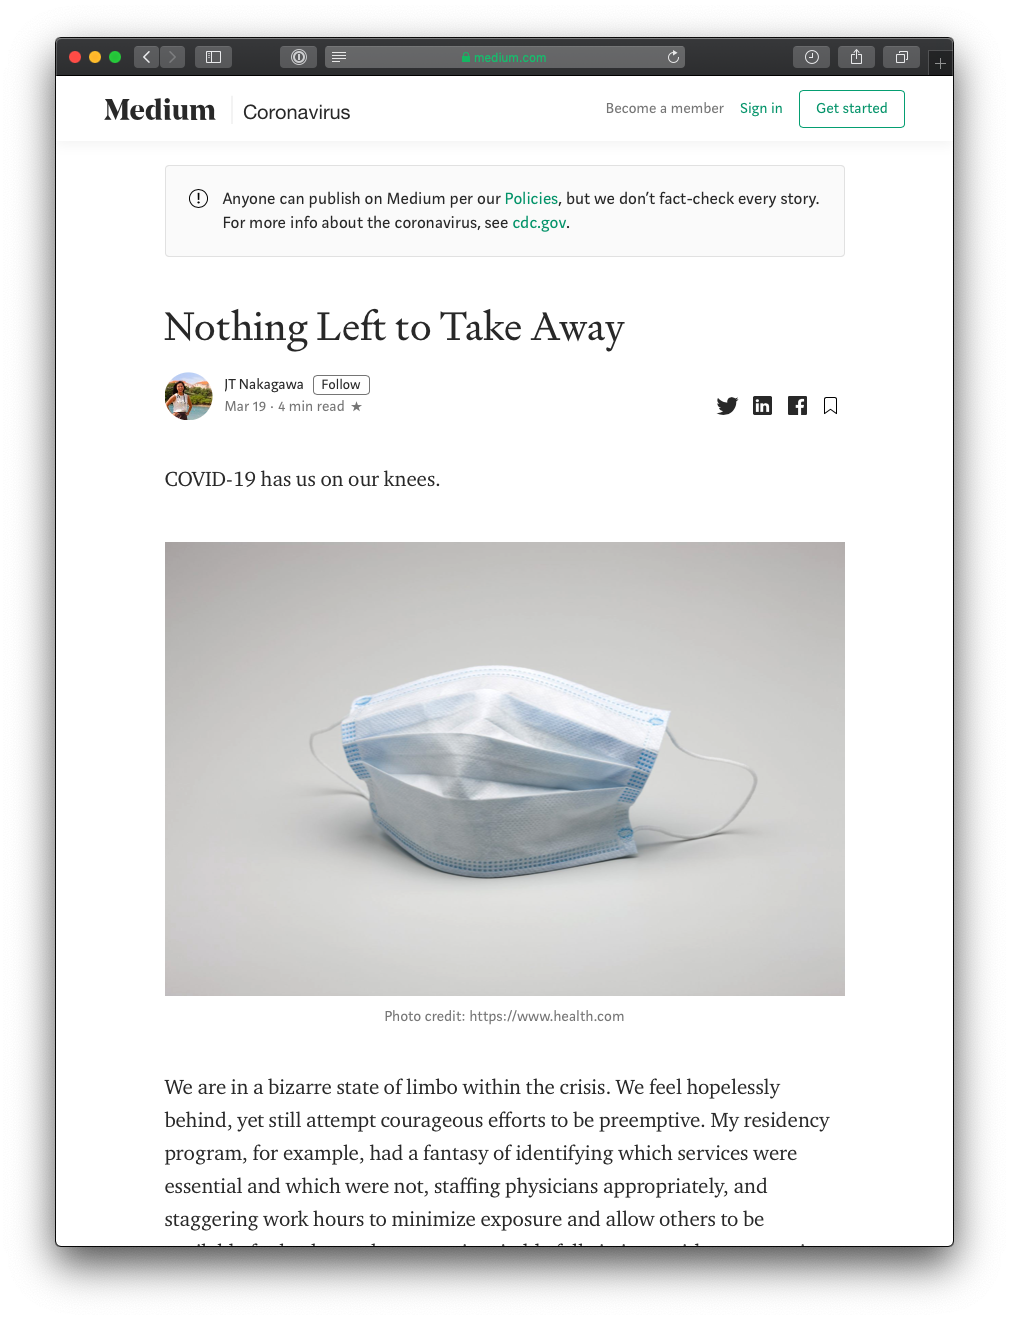
\includegraphics[width=.8\columnwidth]{voorbeeld-medium-desktop}
    \caption[Voorbeeld Medium desktop]{Artikel op Medium weergegeven in een desktop-omgeving}
    \label{fig:ux-voorbeeld-medium:desktop}
\end{figure}

\begin{figure}
    \centering
    \subfloat[Donkere gebruikersomgeving]{{
\includegraphics[width=.4\columnwidth]{voorbeeld-medium-mobiel-donker}}}
    \qquad
    \subfloat[Lichte gebruikersomgeving]{{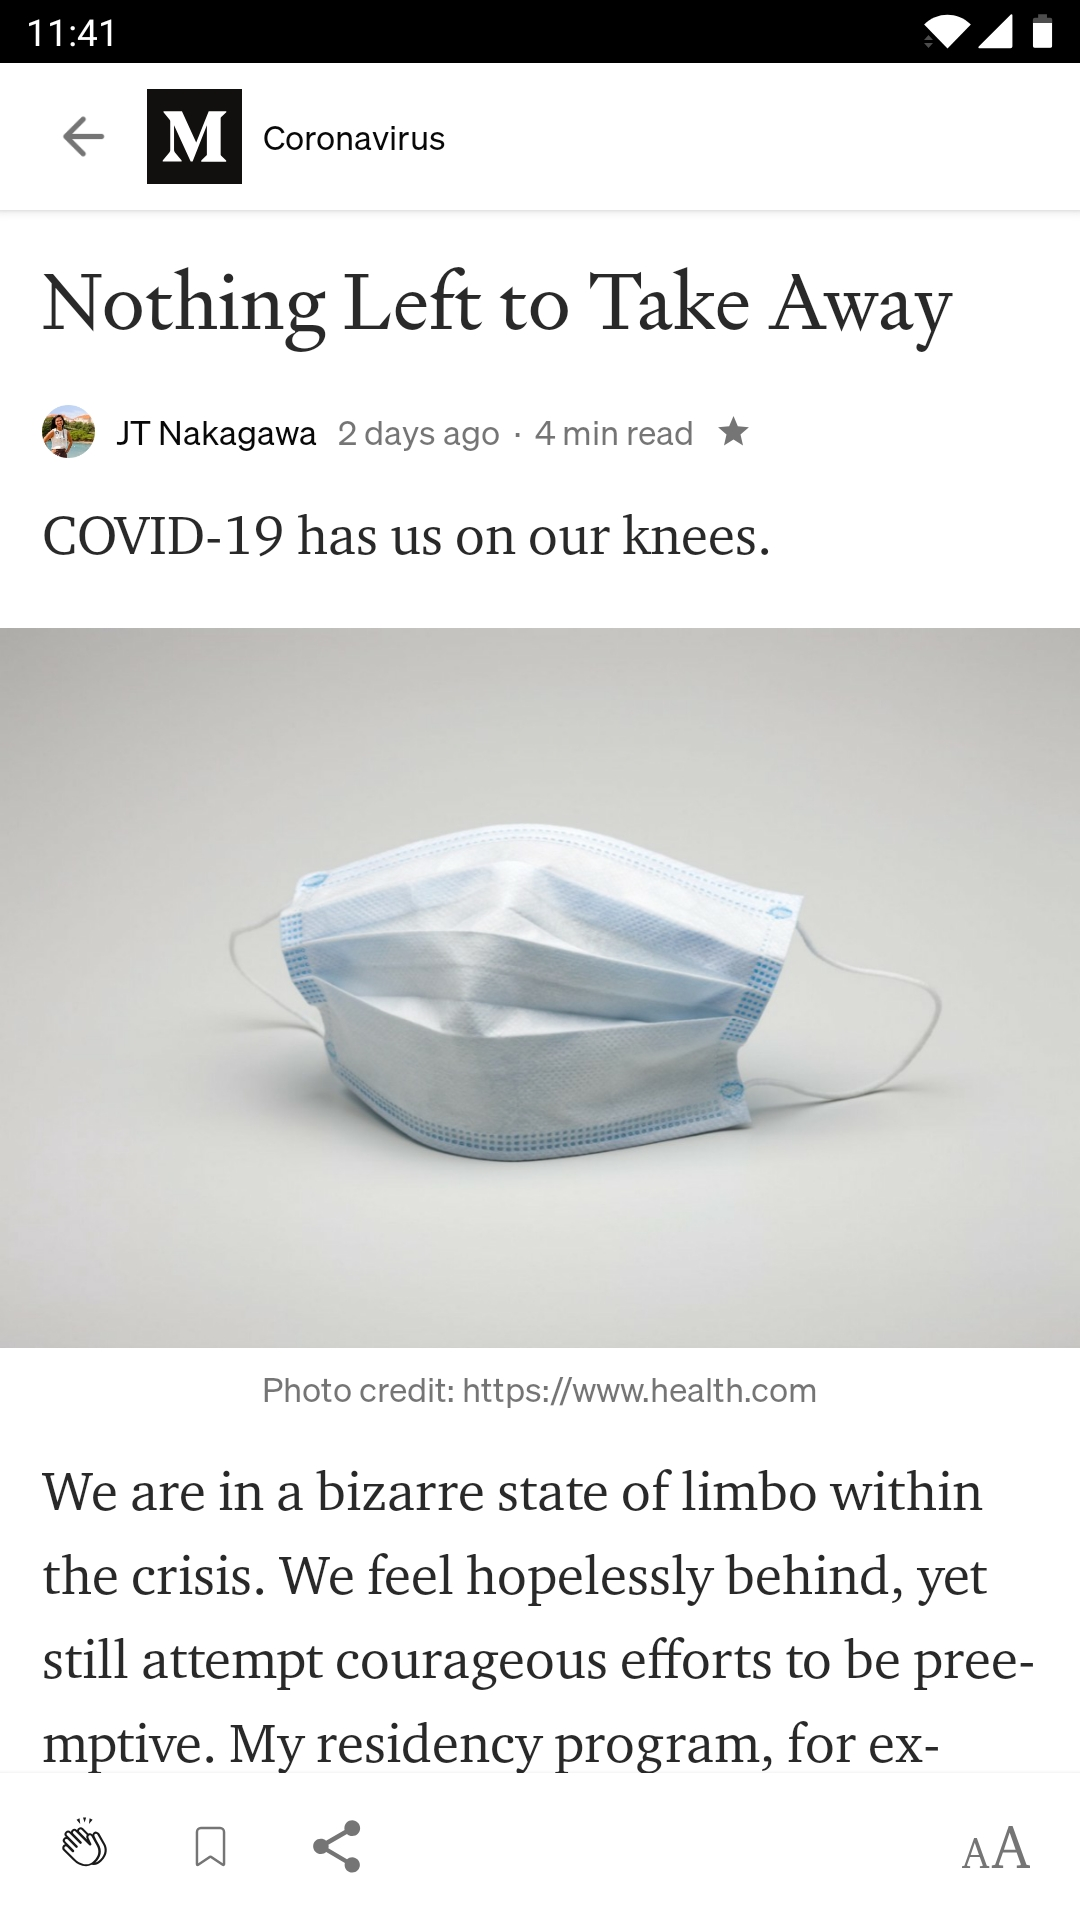
\includegraphics[width=.4\columnwidth]{voorbeeld-medium-mobiel-licht}}}
    \caption[Voorbeeld Medium mobiel]{Artikel op Medium weergegeven in een mobiele omgeving}
    \label{fig:ux-voorbeeld-medium:mobiel}
\end{figure}

\textbf{Airbnb} wil verkopen, dat is merkbaar van zodra je de website opent. Airbnb (\url{https://www.airbnb.com/}) is een platform waarmee je een kamer of woning van iemand anders kan huren voor een korte periode. Het is een razend populair platform bij mensen die een plezier- of werkreis plannen en iets unieks zoeken of de kosten van hun reis willen drukken. Van zodra je op de homepagina komt zorgt Airbnb ervoor dat je onmiddellijk kan zoeken naar een geschikte plaats om te verblijven op een locatie en tijdstip naar keuze. Gepaard met een uitnodigende titel en een buitengewone afbeelding is de verleiding bij de gebruiker groot om hun ideale trip te beginnen plannen. Door deze directe aanpak vergeet de gebruiker als het ware de concurrentie van Airbnb, wat uiteraard net het doel was van bij het begin.

\begin{figure}
    \centering
    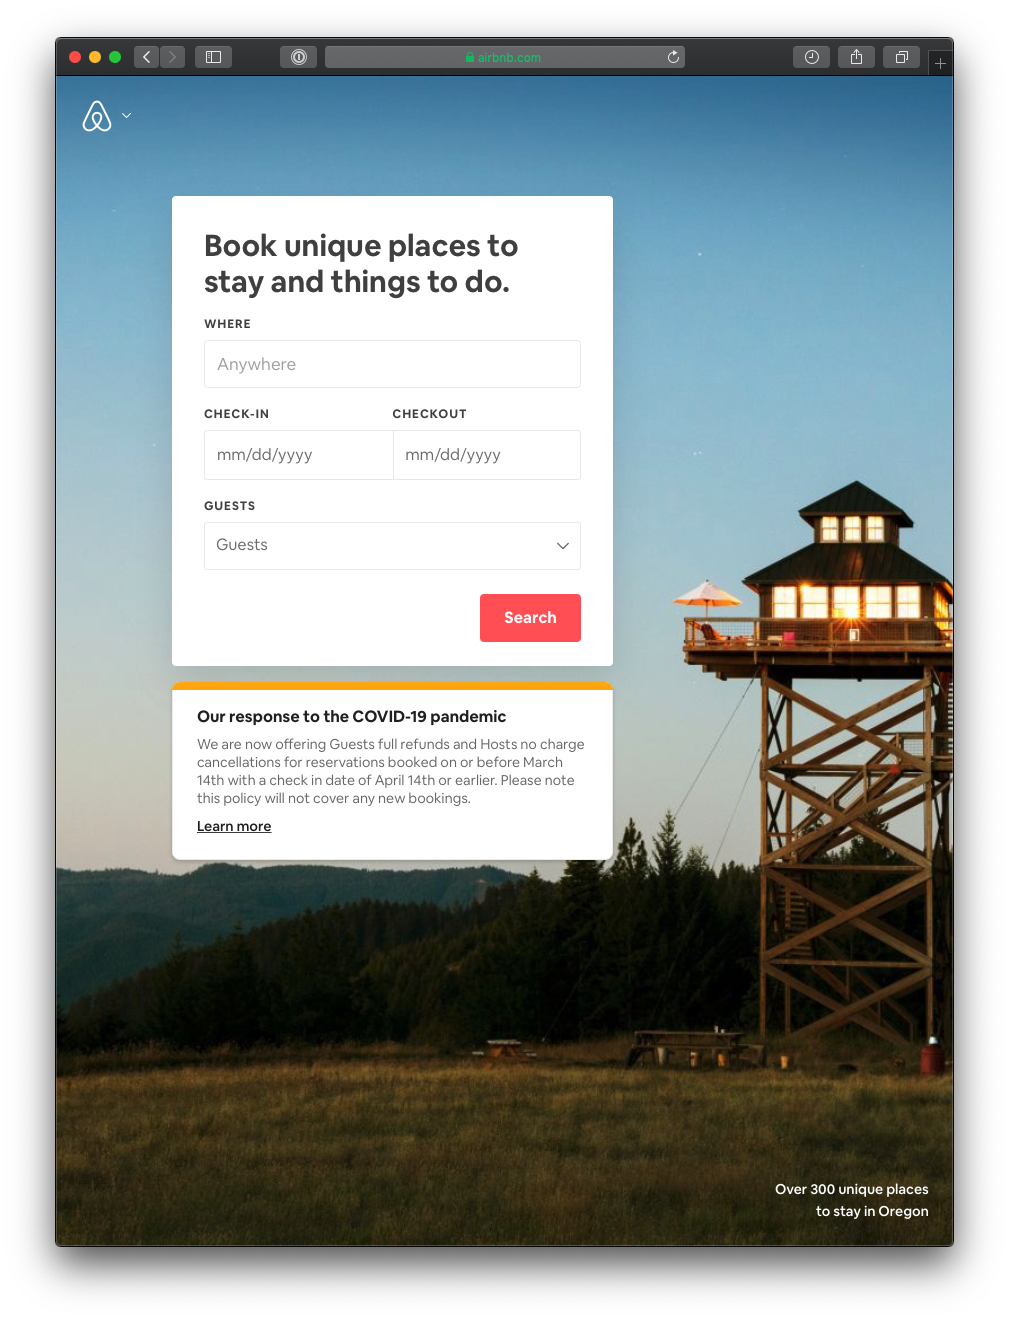
\includegraphics[width=.8\columnwidth]{voorbeeld-airbnb-desktop}
    \caption[Voorbeeld Airbnb]{Airbnb homepagina}
    \label{fig:ux-voorbeeld-airbnb}
\end{figure}

Slimme apparaten in het huishouden zijn bezig aan een opmars. Eén van de bekendste apparaten is de \textbf{Nest Smart Thermostat}, een slimme thermostaat die verbonden is met het internet. De thermostaat leert wanneer de ruimte moet opwarmen of afkoelen. Het fysieke toestel zelf is de simpliciteit zelve. Het is een grote, ronde knop met centraal de huidige temperatuur, hij vermeldt of de ruimtes opwarmen of afkoelen en ook de temperatuur waar men naartoe werkt. Een draai naar rechts en je verhoogt de gewenste temperatuur, een draai naar links en je verlaagt deze. De mobiele applicatie bootst deze werking na zodat de gebruiker zich direct comfortabel voelt met de interface (zie figuur~\ref{fig:ux-voorbeeld-nest}).

\begin{figure}
    \centering
    \subfloat[Fysiek toestel]{{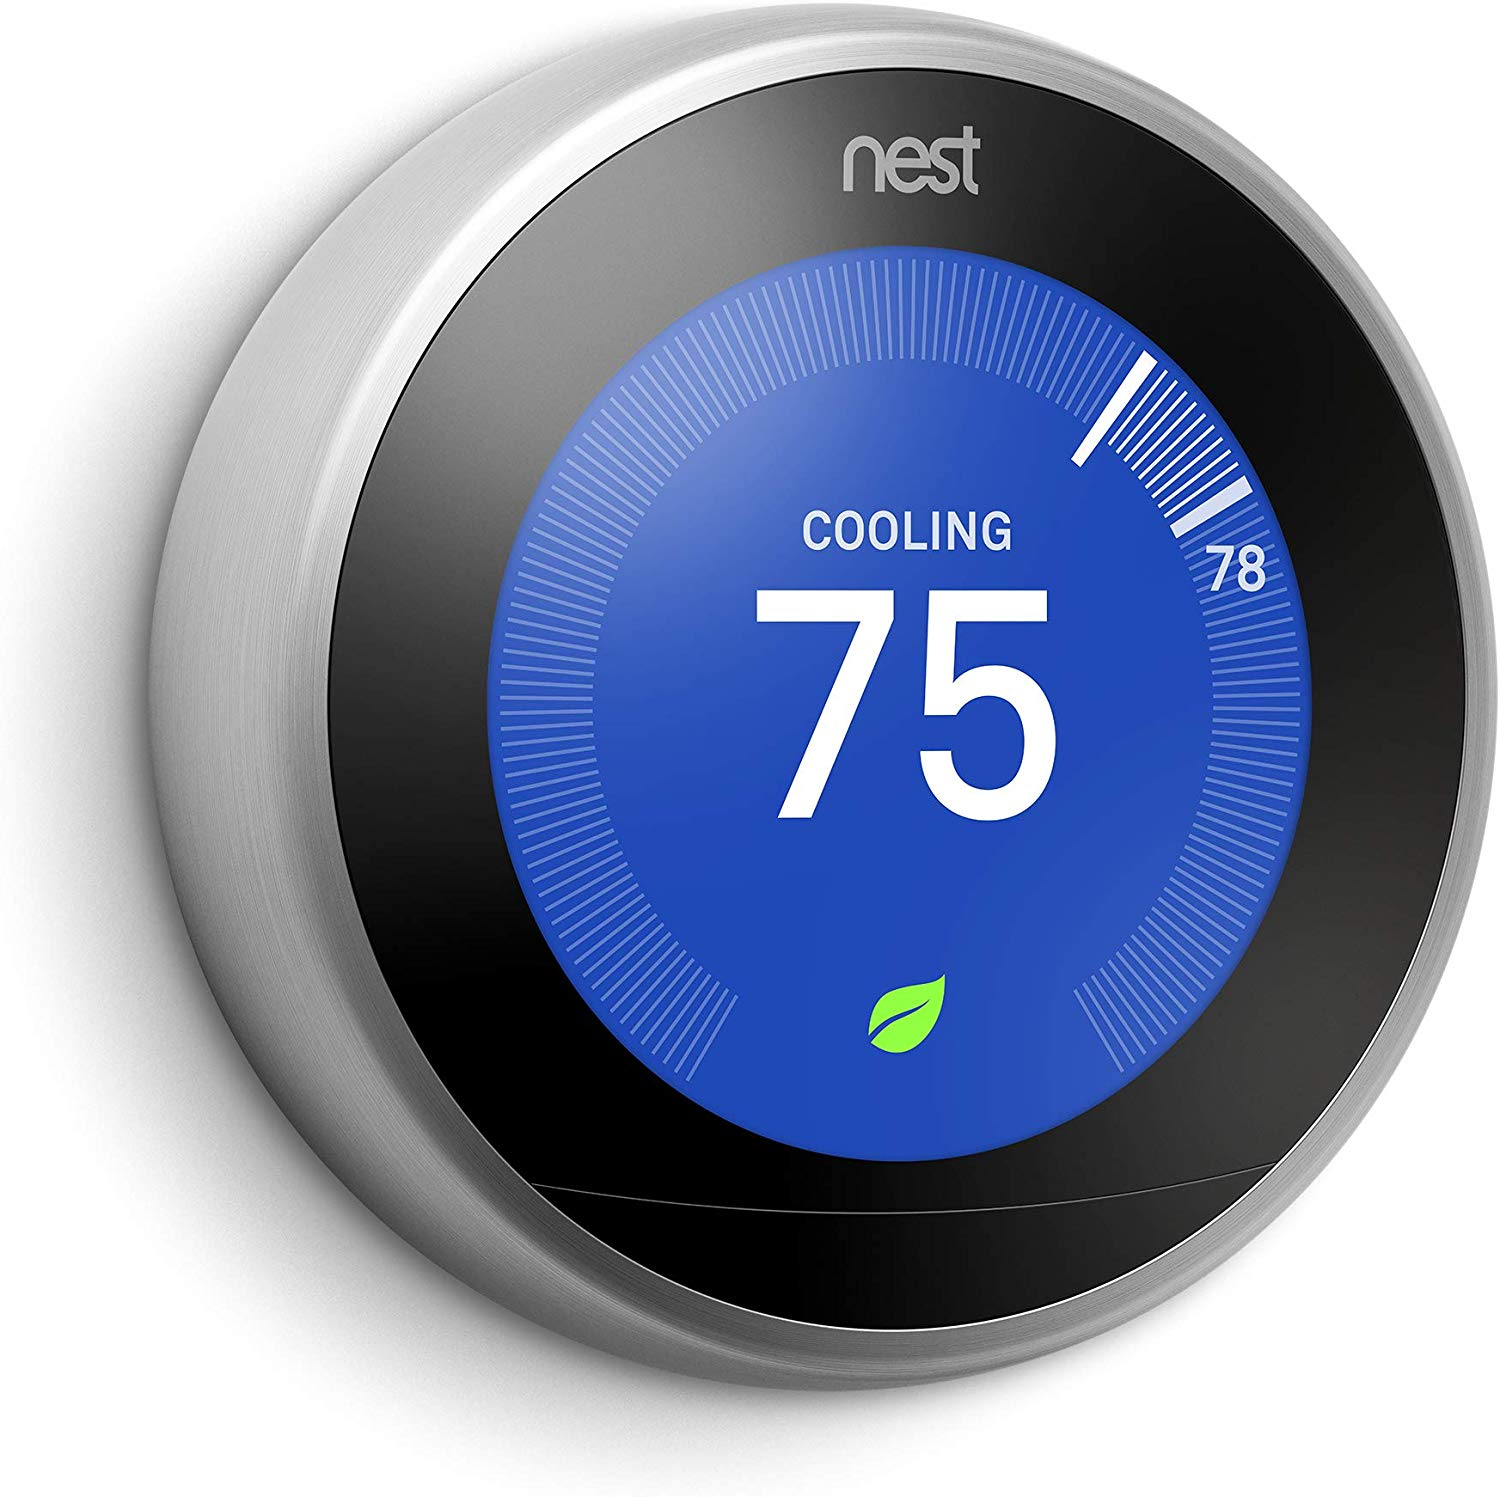
\includegraphics[width=.4\columnwidth]{voorbeeld-nest-toestel}}}
    \qquad
    \subfloat[Mobiele interface]{{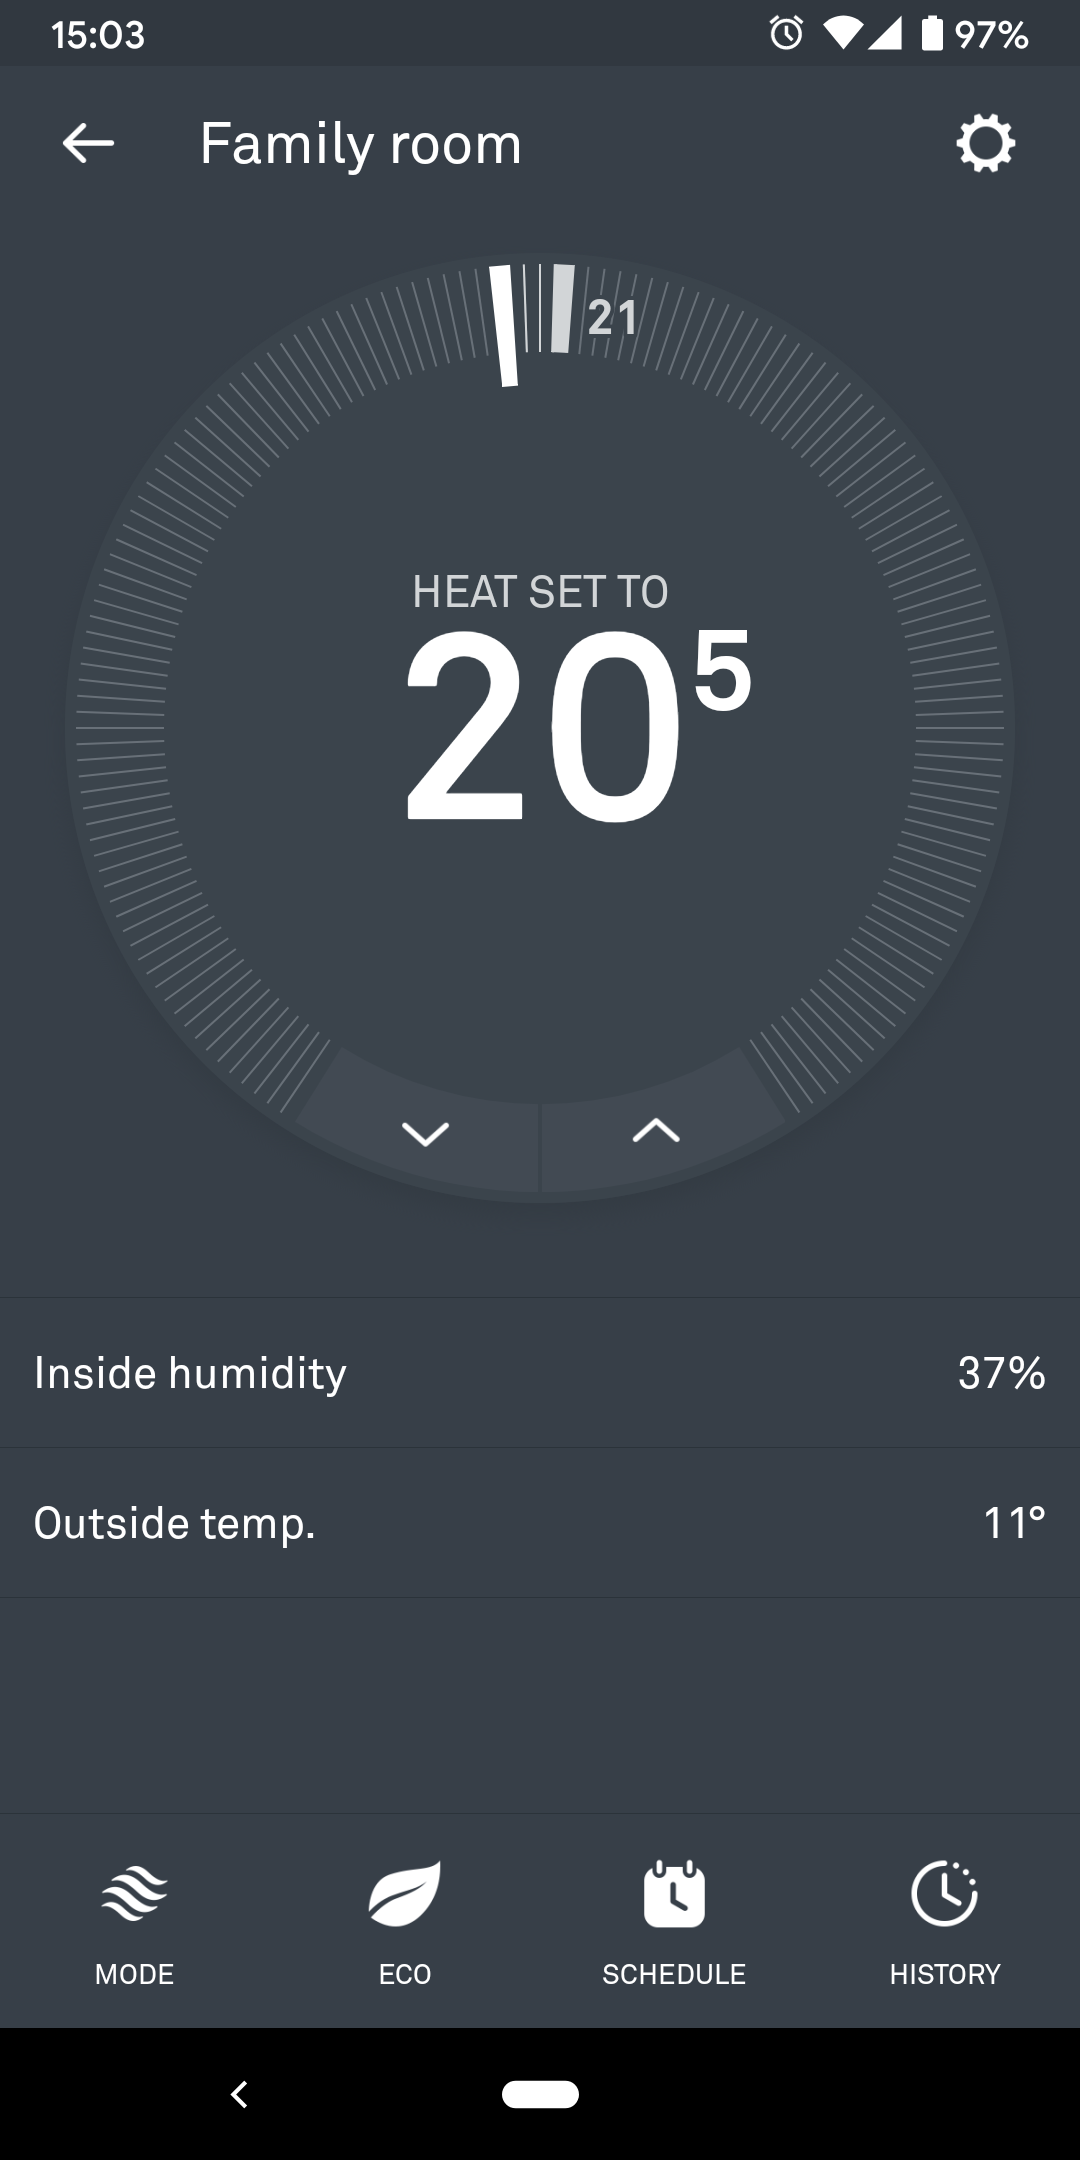
\includegraphics[width=.3\columnwidth]{voorbeeld-nest-mobiel}}}
    \caption[Voorbeeld Nest Smart Thermostat]{Nest Smart Thermostat}
    \label{fig:ux-voorbeeld-nest}
\end{figure}

\textbf{Hubspot} (\url{https://www.hubspot.com/}) maakt producten voor marketing, sales en klantenservice. Hubspot richt zich tot bedrijven van elke omvang. In dit voorbeeld bekijken we slechts een klein deel van de software. Binnen Hubspot is er de mogelijkheid om een massa-e-mail te plannen die een deel van of alle klanten van de gebruiker bereikt. Uiteraard is dit een actie met een aanzienlijke impact op het bedrijf van de gebruiker. Een verzonden e-mail kan echter niet ongedaan gemaakt worden. Wanneer de gebruiker de e-mail inplant komt Hubspot met een pop-up melding die toch nog even bevestiging vraagt (zie figuur~\ref{fig:ux-voorbeeld-hubspot}). Deze melding zorgt ervoor dat de kans op fouten verkleind wordt, maar ook dat de gebruiker zich gerust voelt bij zijn acties.

\begin{figure}
    \centering
    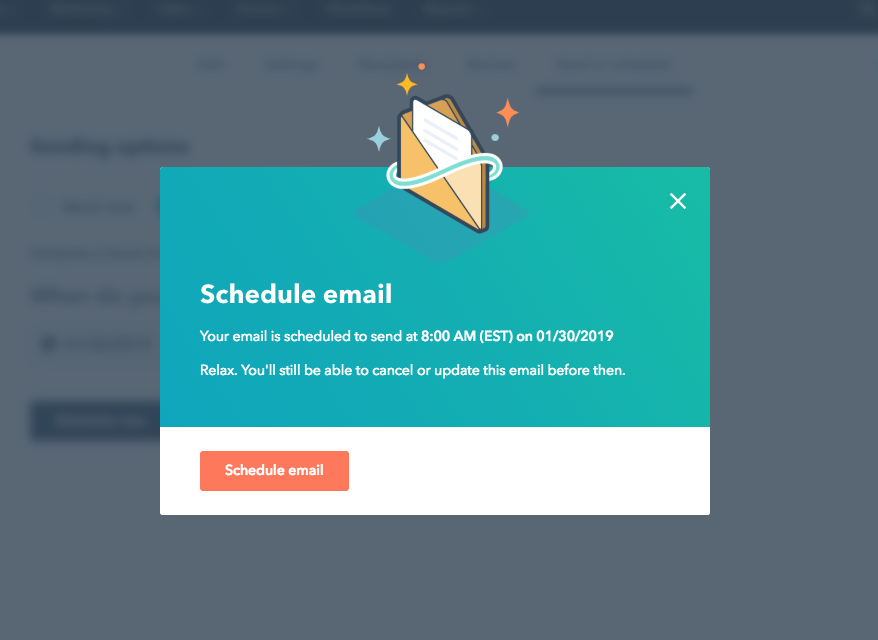
\includegraphics[width=.7\columnwidth]{voorbeeld-hubspot}
    \caption[Voorbeeld Hubspot]{Hubspot pop-up melding}
    \label{fig:ux-voorbeeld-hubspot}
\end{figure}

\section{Usability testing}
\label{sec:usability-testing}

Usability testing is een methode om alle onderdelen van de~\acrlong{acr:ux} honingraat (zie figuur~\ref{fig:ux-facets}) in een applicatie of website te testen. Men test de software in kwestie door er echte gebruikers op te laten werken en ondertussen hun handelingen te observeren. Het doel van usability testing is om de algemene gebruikerservaring te verbeteren~\autocite{Hotjar2020}.

Bij het creëren van software vergeet de ontwikkelaar al snel dat de gewone eindgebruiker vaak meer moeilijkheden zal ondervinden bij het gebruik van zijn creatie dan hijzelf. Doordat de ontwikkelaar hier zelf vaak blind voor is, voert men testen uit met de eindgebruiker. Hierdoor kan men een beter inzicht krijgen over hoe bruikbaar de software is. In dit proces worden vaak vele euvels opgemerkt die anders in de productiesoftware zouden aanbelanden.
Zonder usability testing zou men vaak vast komen te zitten met een product dat door het team van ontwikkelaars wordt begrepen, maar door de doelgroep niet.

In onderstaande testmethoden verwijst men vaak naar het ``think aloud'' protocol. Dit think aloud protocol houdt in dat de deelnemer al zijn of haar acties luidop verklaart. Zo heeft de moderator een beter beeld over de gedachtegang van de deelnemer.

\subsection{Laboratory en field testing}
\label{sec:usability-testing:lab-field-testing}

In voorgaand onderzoek tonen~\textcite{Kaikkonen2005} aan dat usability testing onderverdeeld kan worden in twee categorieën, namelijk laboratory en field testing. Bij field testing worden te testpersonen uitgenodigd om de applicatie in kwestie te testen in de omgeving waar de applicatie normaal zou gebruikt worden. Een mobiele applicatie zoals~\href{https://www.strava.com/}{Strava} die statistieken van lopers en fietsers bijhoudt zou bijvoorbeeld getest worden tijdens een trainingssessie. Sinds de opmars van de smartphone kan field testing steeds meer ingezet worden~\autocite{Kjeldskov2004}. De camera die gebruikt wordt om de testsessie op te nemen wordt steeds kleiner, waardoor het field testing een pak aangenamer wordt.

Laboratory testing houdt in dat men enkele testpersonen uitnodigt in testlabo's, dit is gewoonlijk op kantoor. Dit labo is een rustige ruimte waarin afleidingen beperkt zijn zodat de concentratie gegarandeerd kan worden. Ook al bestaan er veel twijfels rond laboratory testing, volgens \textcite{Kjeldskov2003} wordt het nog steeds vaker verkozen boven field testing. De reden achter deze keuze is vaak omdat men moeilijkheden ondervindt bij field testing. Het is eenvoudiger om testpersonen op te nemen en te observeren bij technieken zoals ``think aloud'' wanneer men gebruik maakt van laboratory testing.

In beide gevallen van usability testing werd geopteerd voor het ``think aloud'' protocol gebaseerd op het werk van~\textcite{Ericsson1984}. Hierbij zal de testpersoon luidop denken. Dit zorgt ervoor dat er veel informatie vrijkomt over de gedachtegang van de gebruiker bij het gebruik van de applicatie. Dit kan makkelijk opgenomen worden om later conclusies uit te trekken.

\textcite{Kaikkonen2005} hebben ook kunnen afleiden dat zowel laboratory testing als field testing quasi dezelfde resultaten vertonen. In hun use case werden alle usability fouten bij beide testmethodes gevonden. Bij field testing vond men de fout soms wel sneller of kwam men deze meerdere keren tegen.

\subsection{Andere testmethoden}
\label{sec:usability-testing:testmethoden}

Laboratory en field testing zijn slecht twee van vele methodes waarmee de bruikbaarheid van een applicatie kan getest worden. In een artikel van~\textcite{Babich2019} worden de zeven belangrijkste methodes opgesomd.

\subsubsection{Guerilla testing}
\label{sec:usability-testing:testmethoden:guerilla}

Guerilla testing is de eenvoudigste testmethode om zo snel mogelijk resultaten te krijgen. Bij guerilla testing gaat de moderator simpelweg op een publieke plaats aan willekeurige personen vragen om even het prototype van de applicatie te gebruiken. De moderator noteert dan de bevindingen. Guerilla testing voert men het best uit in het begin van het ontwikkelproces, zo weet men snel of men in de juiste richting werkt. Vaak krijgt de testpersoon een kleine attentie na het uitvoeren van de test. Zo kan de moderator bijvoorbeeld in een koffiebar plaatsnemen en testpersonen uitnodigen met een gratis koffie.

\subsubsection{Lab usability testing}
\label{sec:usability-testing:testmethoden:lab}

Deze testmethode werd eerder besproken in hoofdstuk~\ref{sec:usability-testing:lab-field-testing}. In contrast met geurilla testing kan men hier een gerichter publiek aantrekken en kan men zo relevantere informatie verkrijgen.

\subsubsection{Unmoderated remote usability testing}
\label{sec:usability-testing:testmethoden:unmoderated-remote}

Dit is een variant van field testing (zie hoofdstuk~\ref{sec:usability-testing:lab-field-testing}) zonder moderator. Hierbij gebruikt de testpersoon de applicatie in zijn omgeving en op zijn toestel. De informatie die men hierdoor verkrijgt is door het gebrek van een moderator uiteraard beperkter. Het voordeel van deze methode is dat de kost lager is dan andere testmethoden.

\subsubsection{Contextual inquiry}
\label{sec:usability-testing:testmethoden:contextual-inquiry}

Deze methode leunt meer aan bij een observatiemethode dan bij een testmethode voor usability testing. De testpersonen krijgen hierbij een lijst met vragen die ze moeten beantwoorden over het product. Achteraf worden ze vaak gevraagd de applicatie te gebruiken in hun omgeving met een moderator (zoals bij field testing).

\subsubsection{Phone interview}
\label{sec:usability-testing:testmethoden:phone}

Deze methode is een variant van laboratory testing waarbij men de testpersoon telefonisch opdrachten geeft. Dit gesprek kan opgenomen worden om later conclusies uit te trekken. Bij deze testmethode worden de communicatievaardigheden van de moderator op proef gesteld.

\subsubsection{Card sorting}
\label{sec:usability-testing:testmethoden:card-sorting}

Hierbij worden alle functionaliteiten van de applicatie op kaartjes geschreven. De testpersoon plaats deze kaarten dan in categorieën en geeft deze kaartjes een bepaalde prioriteit. Van zodra de testpersoon aan het werk gaat met de kaartjes moet de moderator uitleg vragen waarom de testpersoon bepaalde kaartjes op een bepaalde plaats legt. 

\subsubsection{Session recording}
\label{sec:usability-testing:testmethoden:session-recording}

Deze methode legt de acties vast van echte (anonieme) gebruikers. Zo kan men nadien bekijken hoe de sessie bij de gebruiker verlopen is en waar er eventueel~\acrlong{acr:ux} fouten zitten. Ook kan men door deze opnames beter begrijpen welke inhoud en functies belangrijk zijn voor de gebruiker. Deze bevindingen kan men makkelijk aflezen van een heatmap-analyse. Een veelgebruikte tool om sessies op te nemen en heatmap-analyses te generen is~\href{https://www.hotjar.com/}{Hotjar}. Figuur~\ref{fig:testing-hotjar} geeft een voorbeeld van een opname en een heatmap-analyse van de~\href{https://getcardify.com/}{website van Cardify}.

\begin{figure}
    \centering
    \subfloat[Opname handelingen van een gebruiker]{{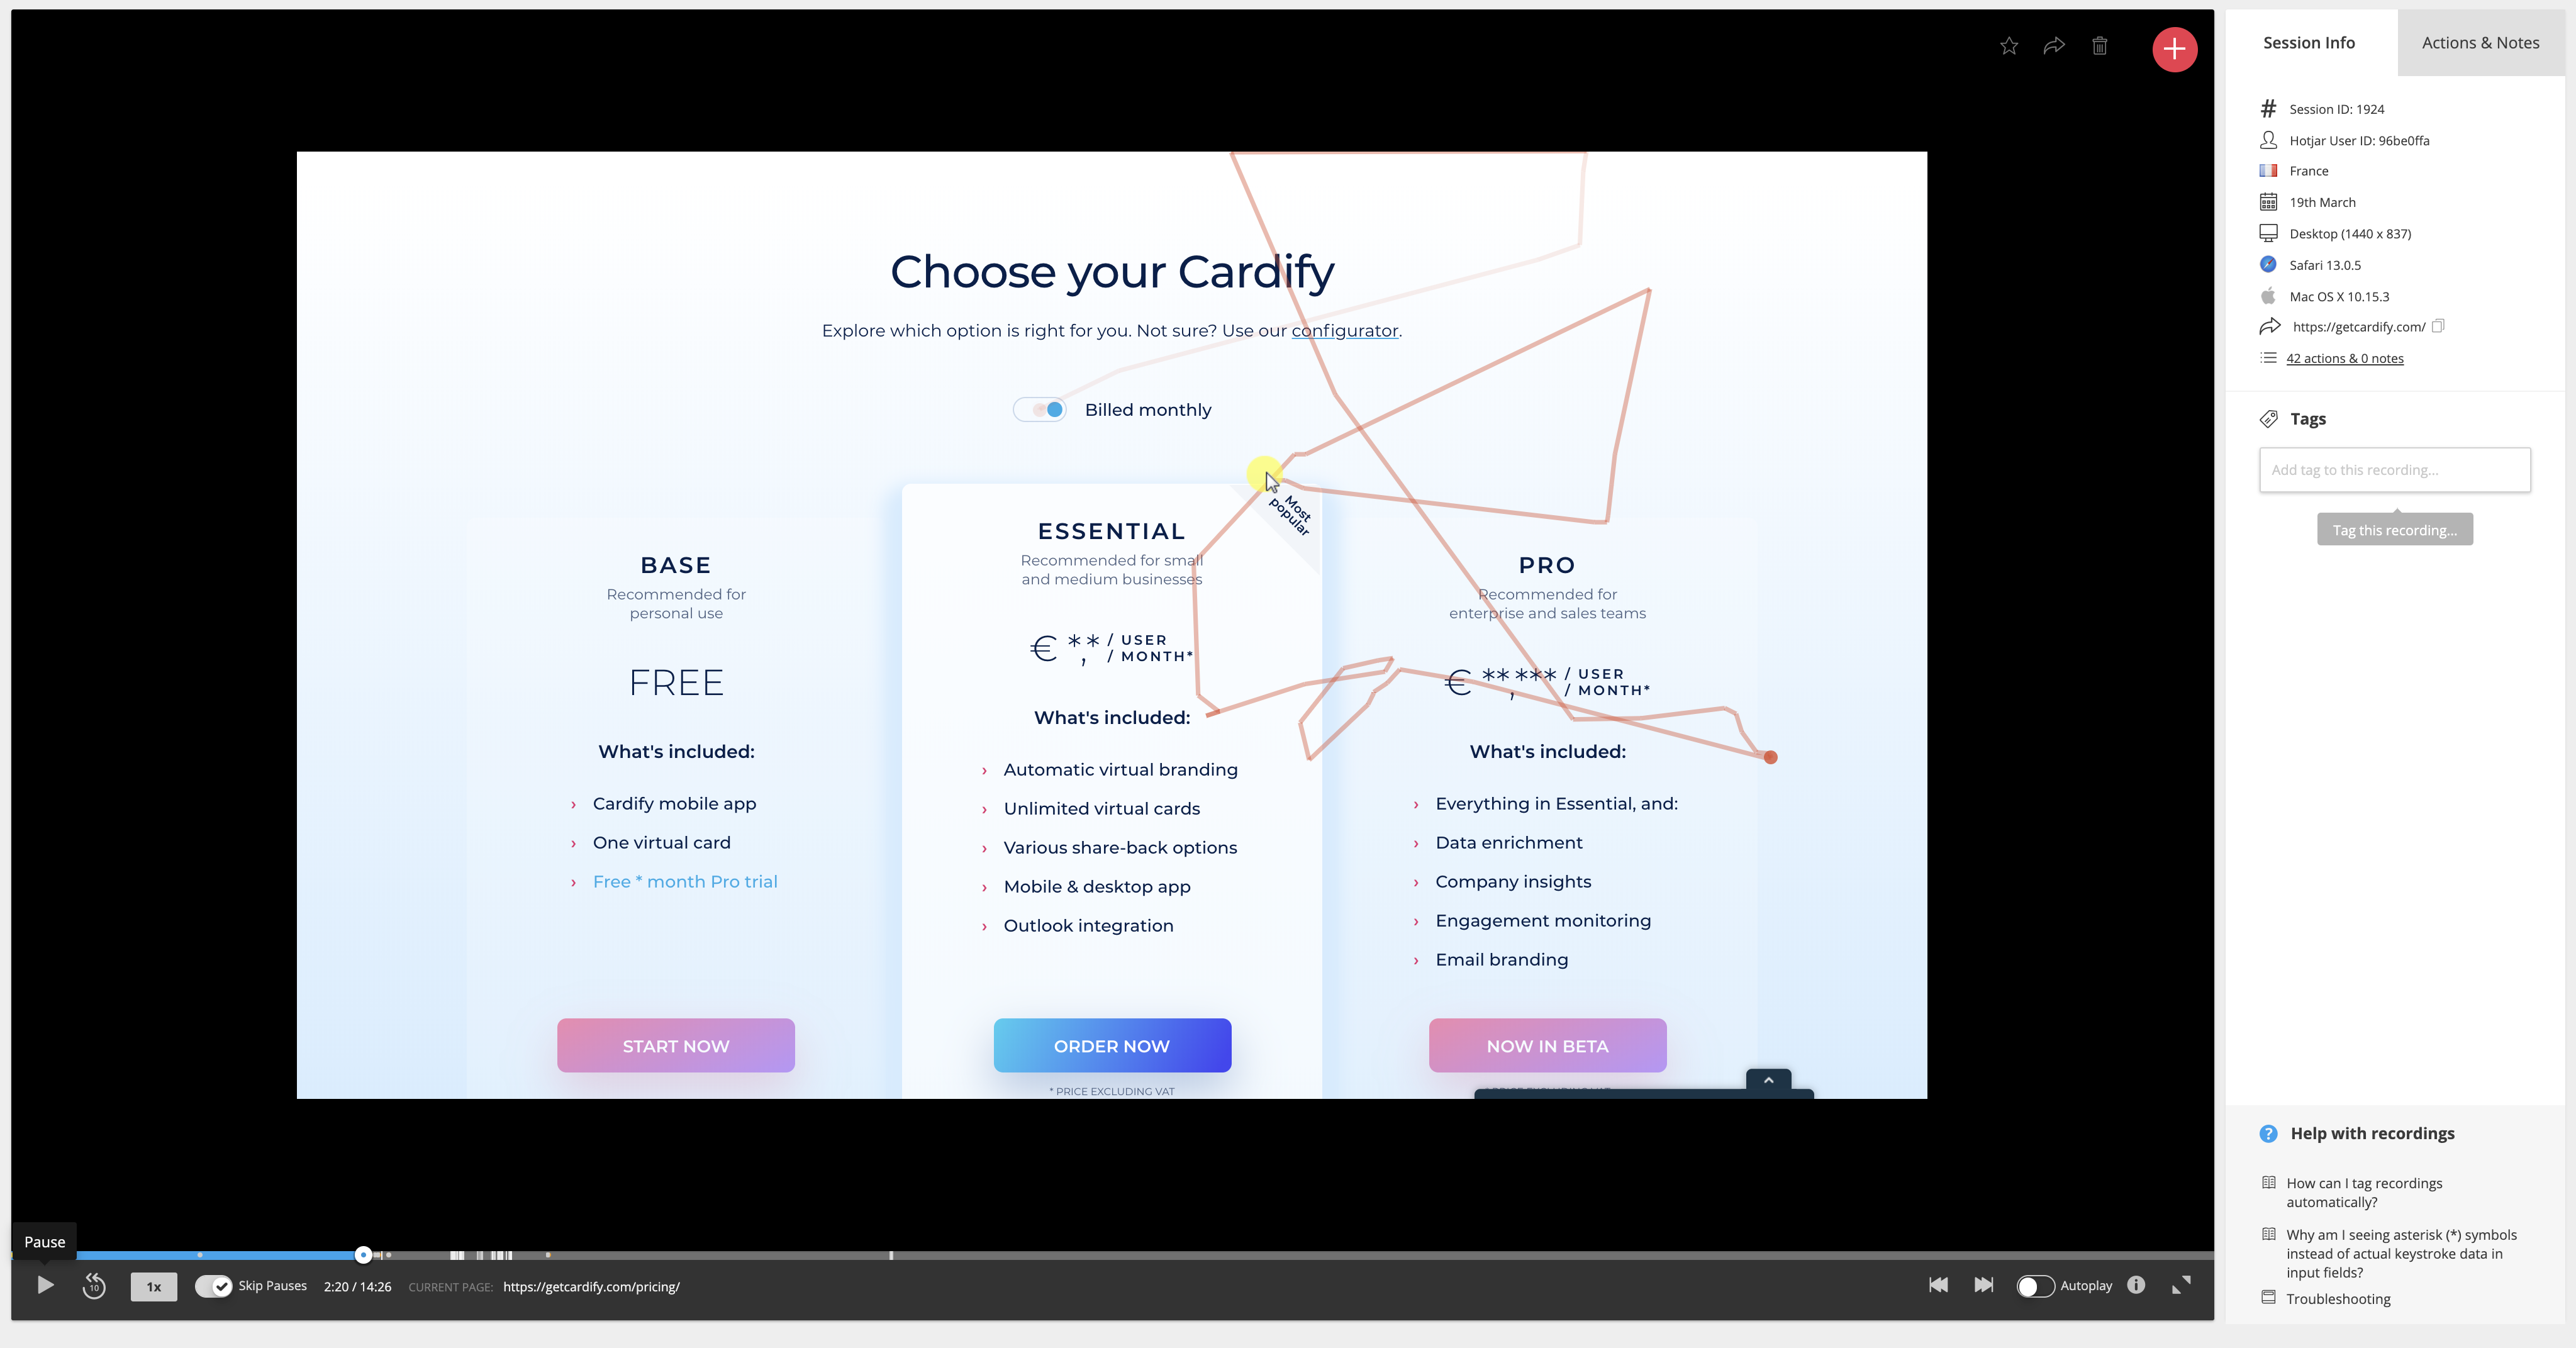
\includegraphics[width=\columnwidth]{voorbeeld-testing-opname}}}
    \qquad
    \subfloat[Heatmap-analyse]{{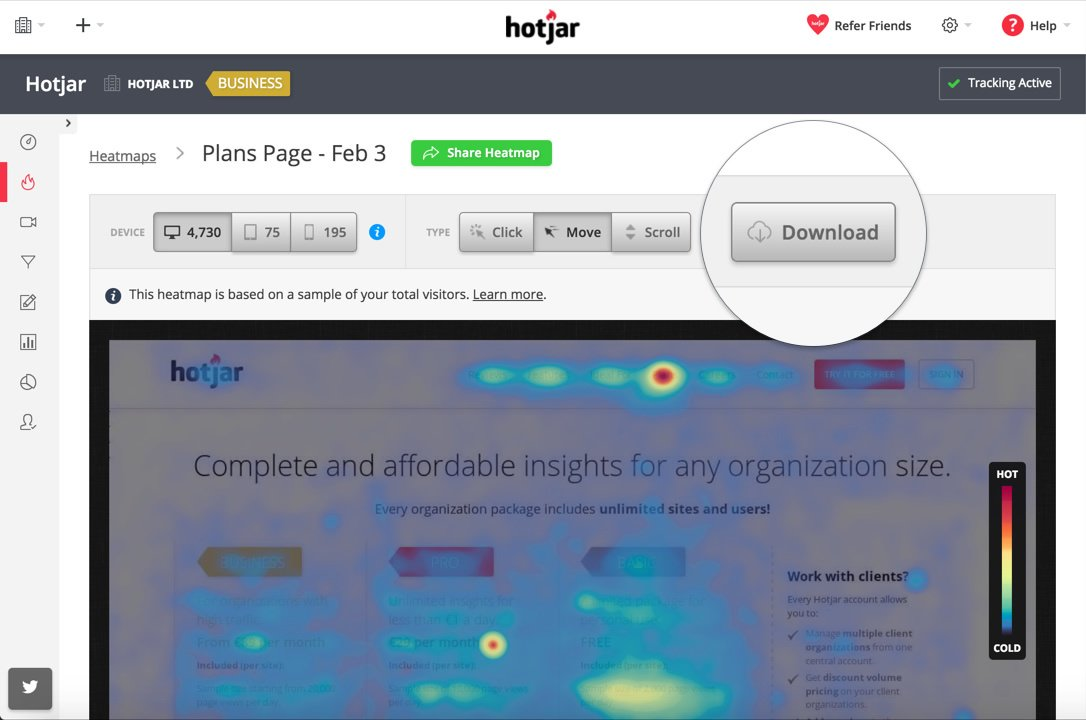
\includegraphics[width=\columnwidth]{voorbeeld-testing-heatmap}}}
    \caption[Voorbeeld session recording]{Voorbeeld session recording bij Cardify}
    \label{fig:testing-hotjar}
\end{figure}

\subsection{Testpersonen}
\label{sec:usability-testing:testpersonen}

De testpersonen bij usability testing moeten zorgvuldig gekozen worden. De doelgroep moet nauwkeurig vastgelegd worden. Zo zal een bejaarde dame geen meerwaarde bieden bij een applicatie gericht op schoolgaande jeugd. In onderzoek van~\textcite{Alnashri2016} bekijkt men ook de verschillen tussen introverte en extroverte personaliteiten.

Zoals~\textcite{Faulkner2003} aanhaalde heeft het weinig nut om honderden testpersonen te zoeken. Twintig personen zou volstaan om 95\% van de usability problemen op te merken.

In voorgaand onderzoek van~\textcite{Marcus2006} toont men aan dat er culturele verschillen een grote invloed hebben op~\acrshort{acr:ux}. Hieruit kunnen we concluderen dat variëteit in de testpersonen zal lonen.

\subsection{De~\acrlong{acr:sus}}
\label{sec:usability-testing:sus}

De~\acrlong{acr:sus} is een snelle manier om, met behulp van een vragenlijst, te weten te komen of de usability van het product goed zit. De vragenlijst bestaat uit tien vragen met telkens vijf antwoordmogelijkheden; gaande van ``helemaal mee eens'' tot ``helemaal niet mee eens''. Voor de testpersonen is dit eenvoudig in te vullen. De berekening nadien is echter complex.

Bijgevoegd aan deze scriptie is een template voor de~\acrlong{acr:sus}~\autocite{Calisto2018} (zie bijlage~\ref{bijlage:sus}).

In deze vragenlijst bevinden zich twee vragen die testen op learnability in plaats van op usability~\autocite{Lewis2009}.

\section{Learnability}
\label{sec:learnability}

Er is nog steeds een verschil tussen hoe bruikbaar een applicatie is en hoe goed de eindgebruiker deze applicatie kent. \textcite{Coyle2016} merkten op dat naast de bruikbaarheid (usability) van hun ontwerpen, er ook moest gekeken worden naar de leerbaarheid (learnability) ervan. Na een hele reeks testen en vragenlijsten met gebruikers uit de doelgroep kon men effectief afleiden dat, indien de leerbaarheid van een applicatie ook in acht genomen wordt, men diepere gebruiksproblemen gemakkelijker kon vaststellen. Bij hun onderzoek maakten ze gebruik van onder andere open vragen, de~\acrlong{acr:sus} (zie hoofdstuk~\ref{sec:usability-testing:sus}) en vertrouwensratings gebruikmakend van de Likert schaal.

In onderzoek van~\textcite{Haramundanis2001} werd beschreven welke stappen men moest ondernemen om leerbare materie te ontwikkelen:
\begin{itemize}
    \item Analytisch denken
    \item Logische ontwikkeling
    \item Usability testen
    \item Consistentie van aanpak
    \item Visualisatie
\end{itemize}

Visualisatie is hierbij een belangrijk onderdeel. In de beginjaren van de personal computer moest men nog door de mappenstructuur van het besturingssysteem bladeren met behulp van de~\acrlong{acr:cli}. De leercurve was toen uiteraard zeer steil waardoor de computer een product was waarmee weinig mensen mee overweg konden. Tegenwoordig kan iedereen door zijn of haar mappen bladeren in een besturingssysteem door middel van een~\acrlong{acr:gui}. Deze verandering bij het gebruik van de personal computer zorgde er ook voor dat het gebruik van een computer makkelijk aan te leren was voor nieuwe gebruikers. Deze evolutie in het ontwerp van software zorgde ervoor dat bijna elk modern huishouden een computer ter beschikking heeft.

\begin{figure}[h]
    \centering
    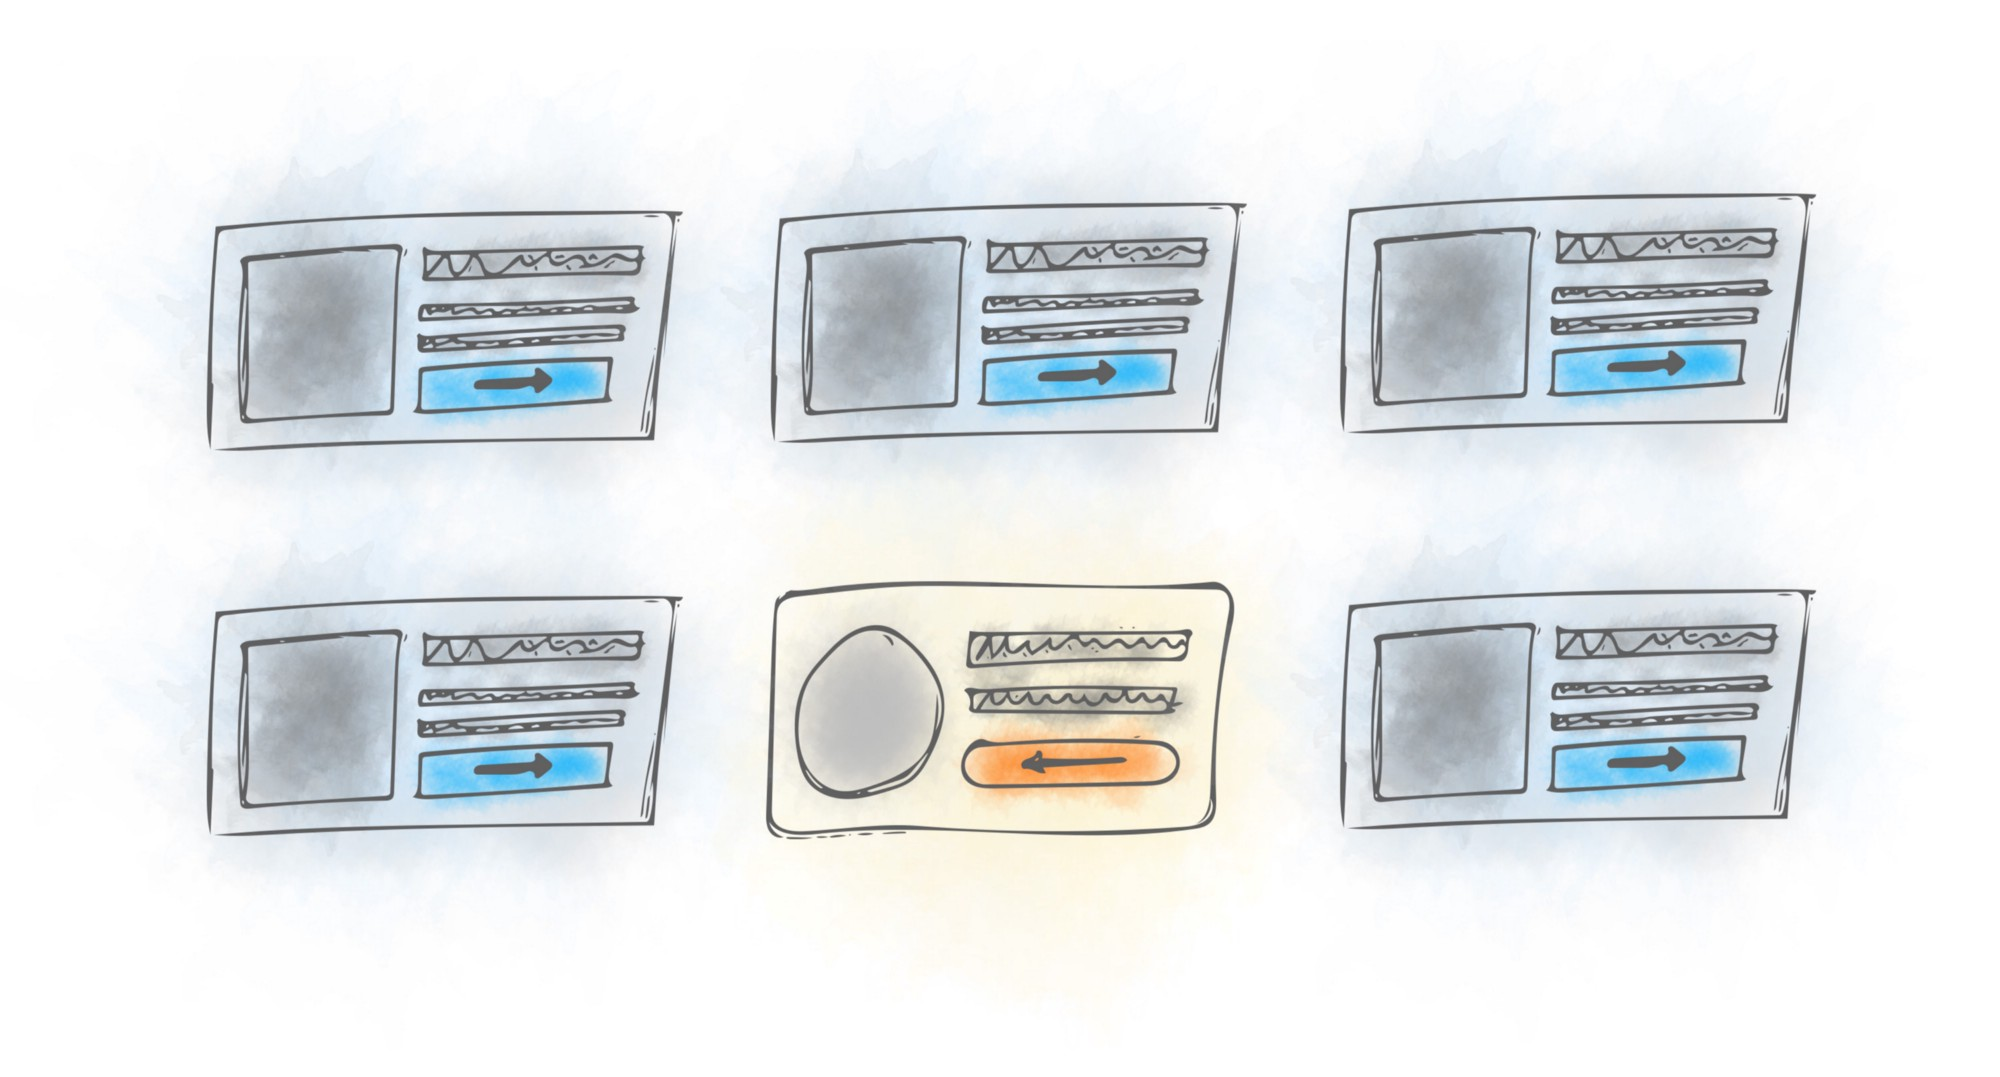
\includegraphics[width=.5\columnwidth]{consistency-sketch}
    \caption[Consistentie doorheen~\acrshort{acr:ui}-elementen]{Het belang van consistentie doorheen~\acrshort{acr:ui}-elementen}
    \label{fig:learnability:consistentie}
\end{figure}

Ook consistentie is belangrijk bij zowel learnability als~\acrshort{acr:ux} design. Zoals~\textcite{Nikolov2017} aangeeft is bestaan er vier verschillende types van consistentie: visuele, functionele, interne en externe consistentie. De visuele consistentie (zie figuur~\ref{fig:learnability:consistentie}) leunt aan bij het hiervoor genoemde visualisatie. Interne consistentie is een combinatie van visuele en functionele consistentie. Bij het behouden van interne consistentie kan men makkelijk een nieuwe functionaliteit of~\acrshort{acr:ui}-element toevoegen aan bestaande software zonder dat eindgebruikers opnieuw moeten bijleren hoe de applicatie werkt. Externe consistentie trekt de lijn door naar andere systemen en producten. Bij Cardify blijft men consistent doorheen hun volledige aanbod aan producten (zie figuur~\ref{fig:learnability:consistentie-cardify}). Zo zal een gebruiker van de mobiele applicatie zich snel vertrouwd voelen met de verscheidene webplatformen die Cardify te bieden heeft. Vaak gebruikt een bedrijf ook design guidelines. Grote bedrijven zoals Google gaan daarin natuurlijk wat verder. Zo ontwikkelde Google het \href{https://material.io/}{Material Design} systeem. Bij Cardify kan je de design guidelines vinden op \url{https://getcardify.com/brand/}.

\begin{figure}
    \centering
    \subfloat[Web-platform]{{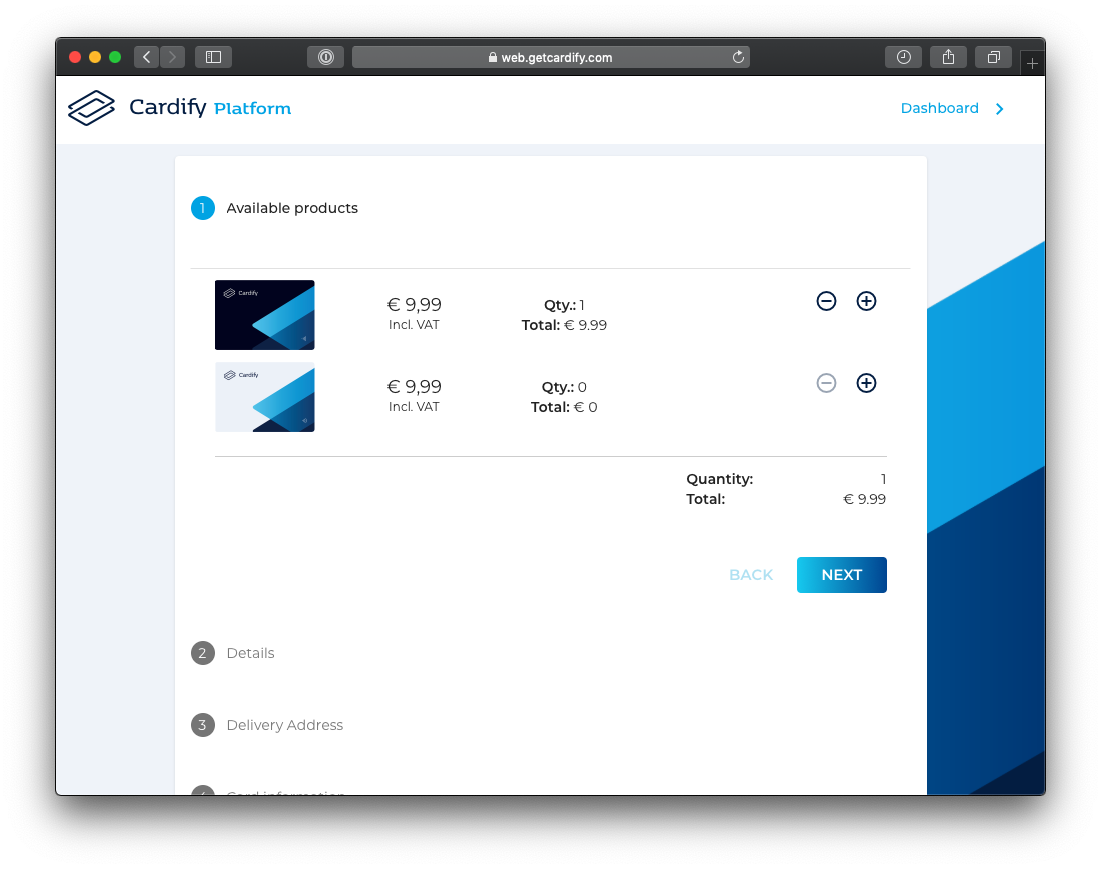
\includegraphics[width=.65\columnwidth]{cardify-consistency-web}}}
    \qquad
    \subfloat[Mobiele applicatie]{{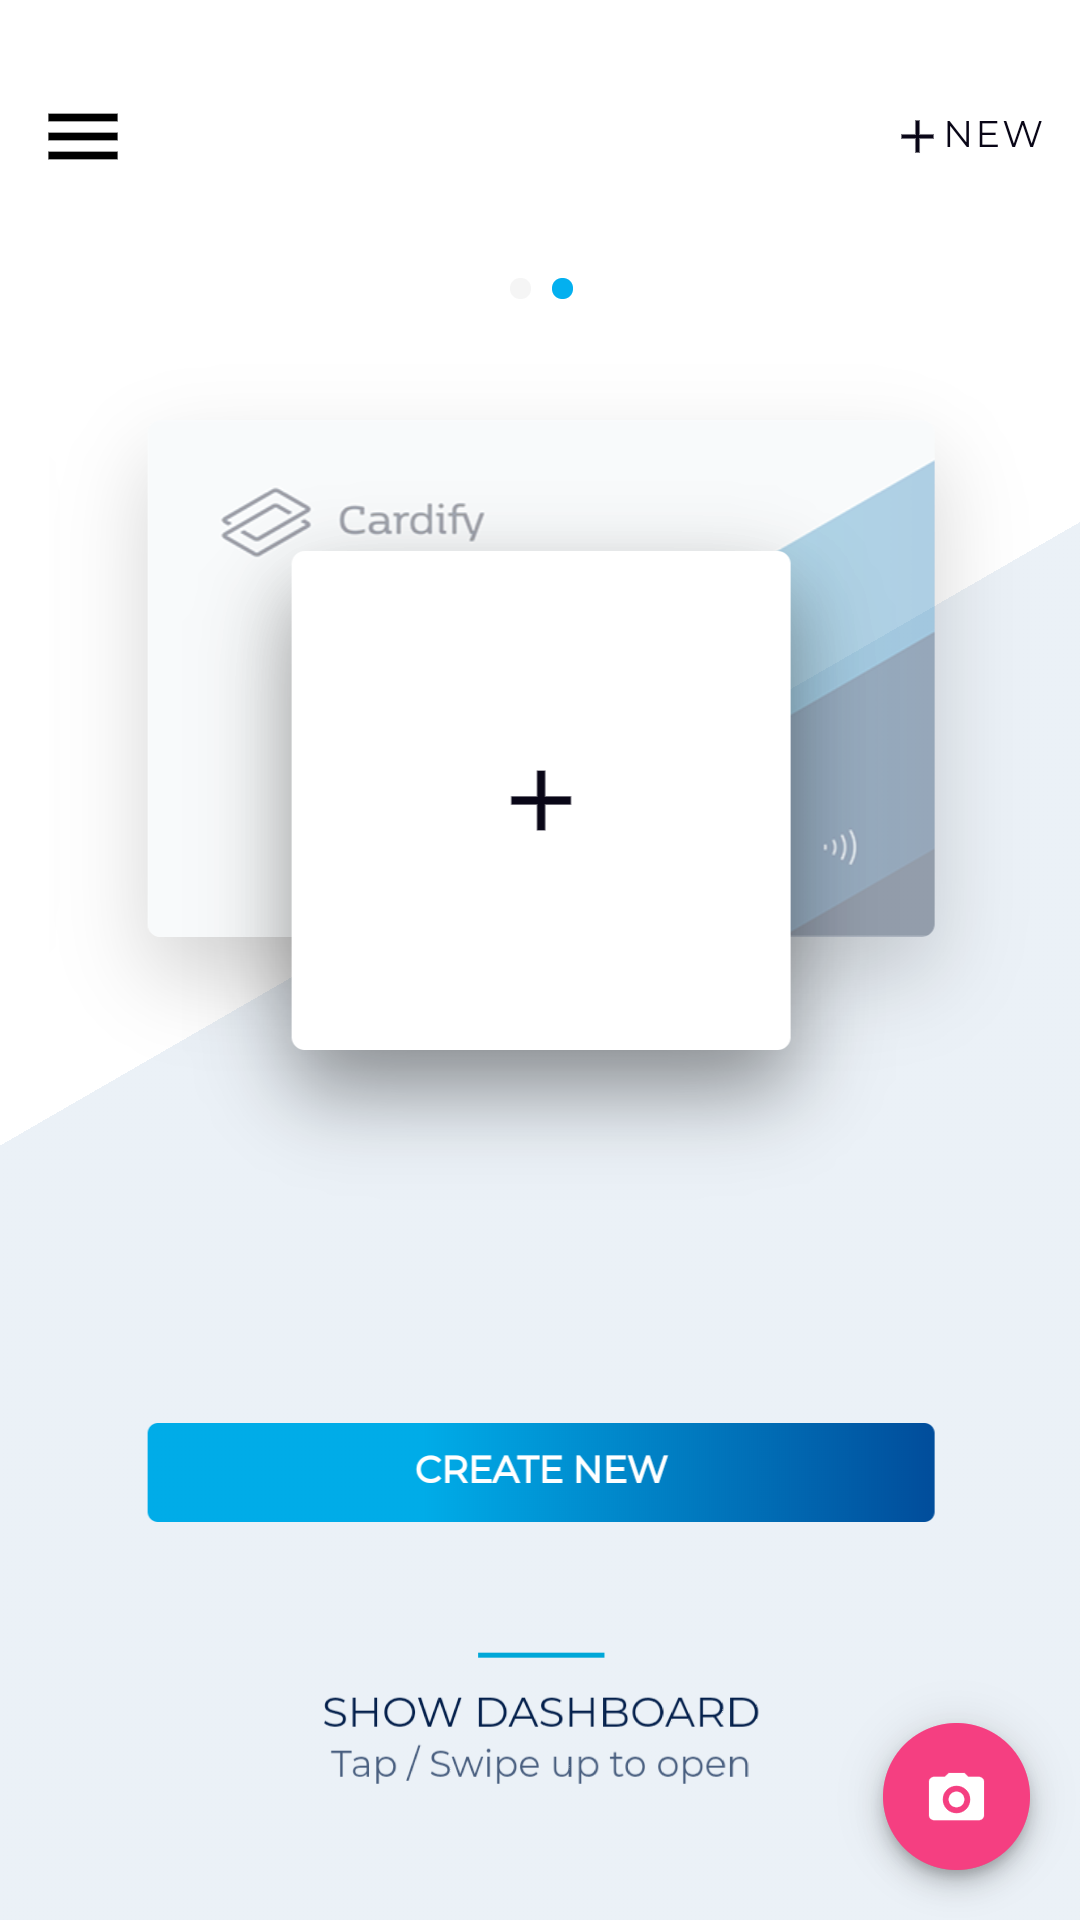
\includegraphics[width=.29\columnwidth]{cardify-consistency-app}}}
    \caption{Consistentie doorheen Cardify producten}
    \label{fig:learnability:consistentie-cardify}
\end{figure}

\section{Onboarding}
\label{sec:onboarding}

Onboarding is slechts één element van de velen die de~\acrlong{acr:ux} in software kunnen beïnvloeden. Het is echter wel één van de bekendste en belangrijkste. Voorgaand onderzoek toonde aan hoe onboarding een positieve invloed had op de tevredenheid van de gebruiker over de applicatie~\autocite{Cardoso2017}. Onboarding vindt plaats wanneer de gebruiker de applicatie voor de eerste maal opstart en gebruikt. Het is een soort van gids die de gebruiker de belangrijkste functionaliteiten van de applicatie laat zijn. Vaak wordt onboarding ook ingezet voor het verkrijgen van essentiële informatie van de gebruiker, bijvoorbeeld wanneer deze een account moet aanmaken.

Een onboarding kan de ervaring van de gebruiker zeer positief beïnvloeden. Een slecht geïmplementeerde onboarding kan de ervaring weliswaar heel snel negatief beïnvloeden. Er mag dus zeker niet overdreven worden.

Voorgaand onderzoek~\autocite{Desai2019} toonde aan dat een goed geïmplementeerde onboarding (een onboarding gebaseerd op wat de gebruiker wil bereiken) wel degelijk een heleboel voordelen te bieden heeft. Zo zijn klanten met een positieve perceptie minder geneigd om te stoppen met het gebruik van de applicatie in de eerst 21 dagen dat ze klant zijn. In ideale omstandigheden stijgt de bereidheid om te betalen voor de software met 27\%, wat dus resulteert in een gunstigere~\acrfull{acr:roi}.

\begin{figure}
    \centering
    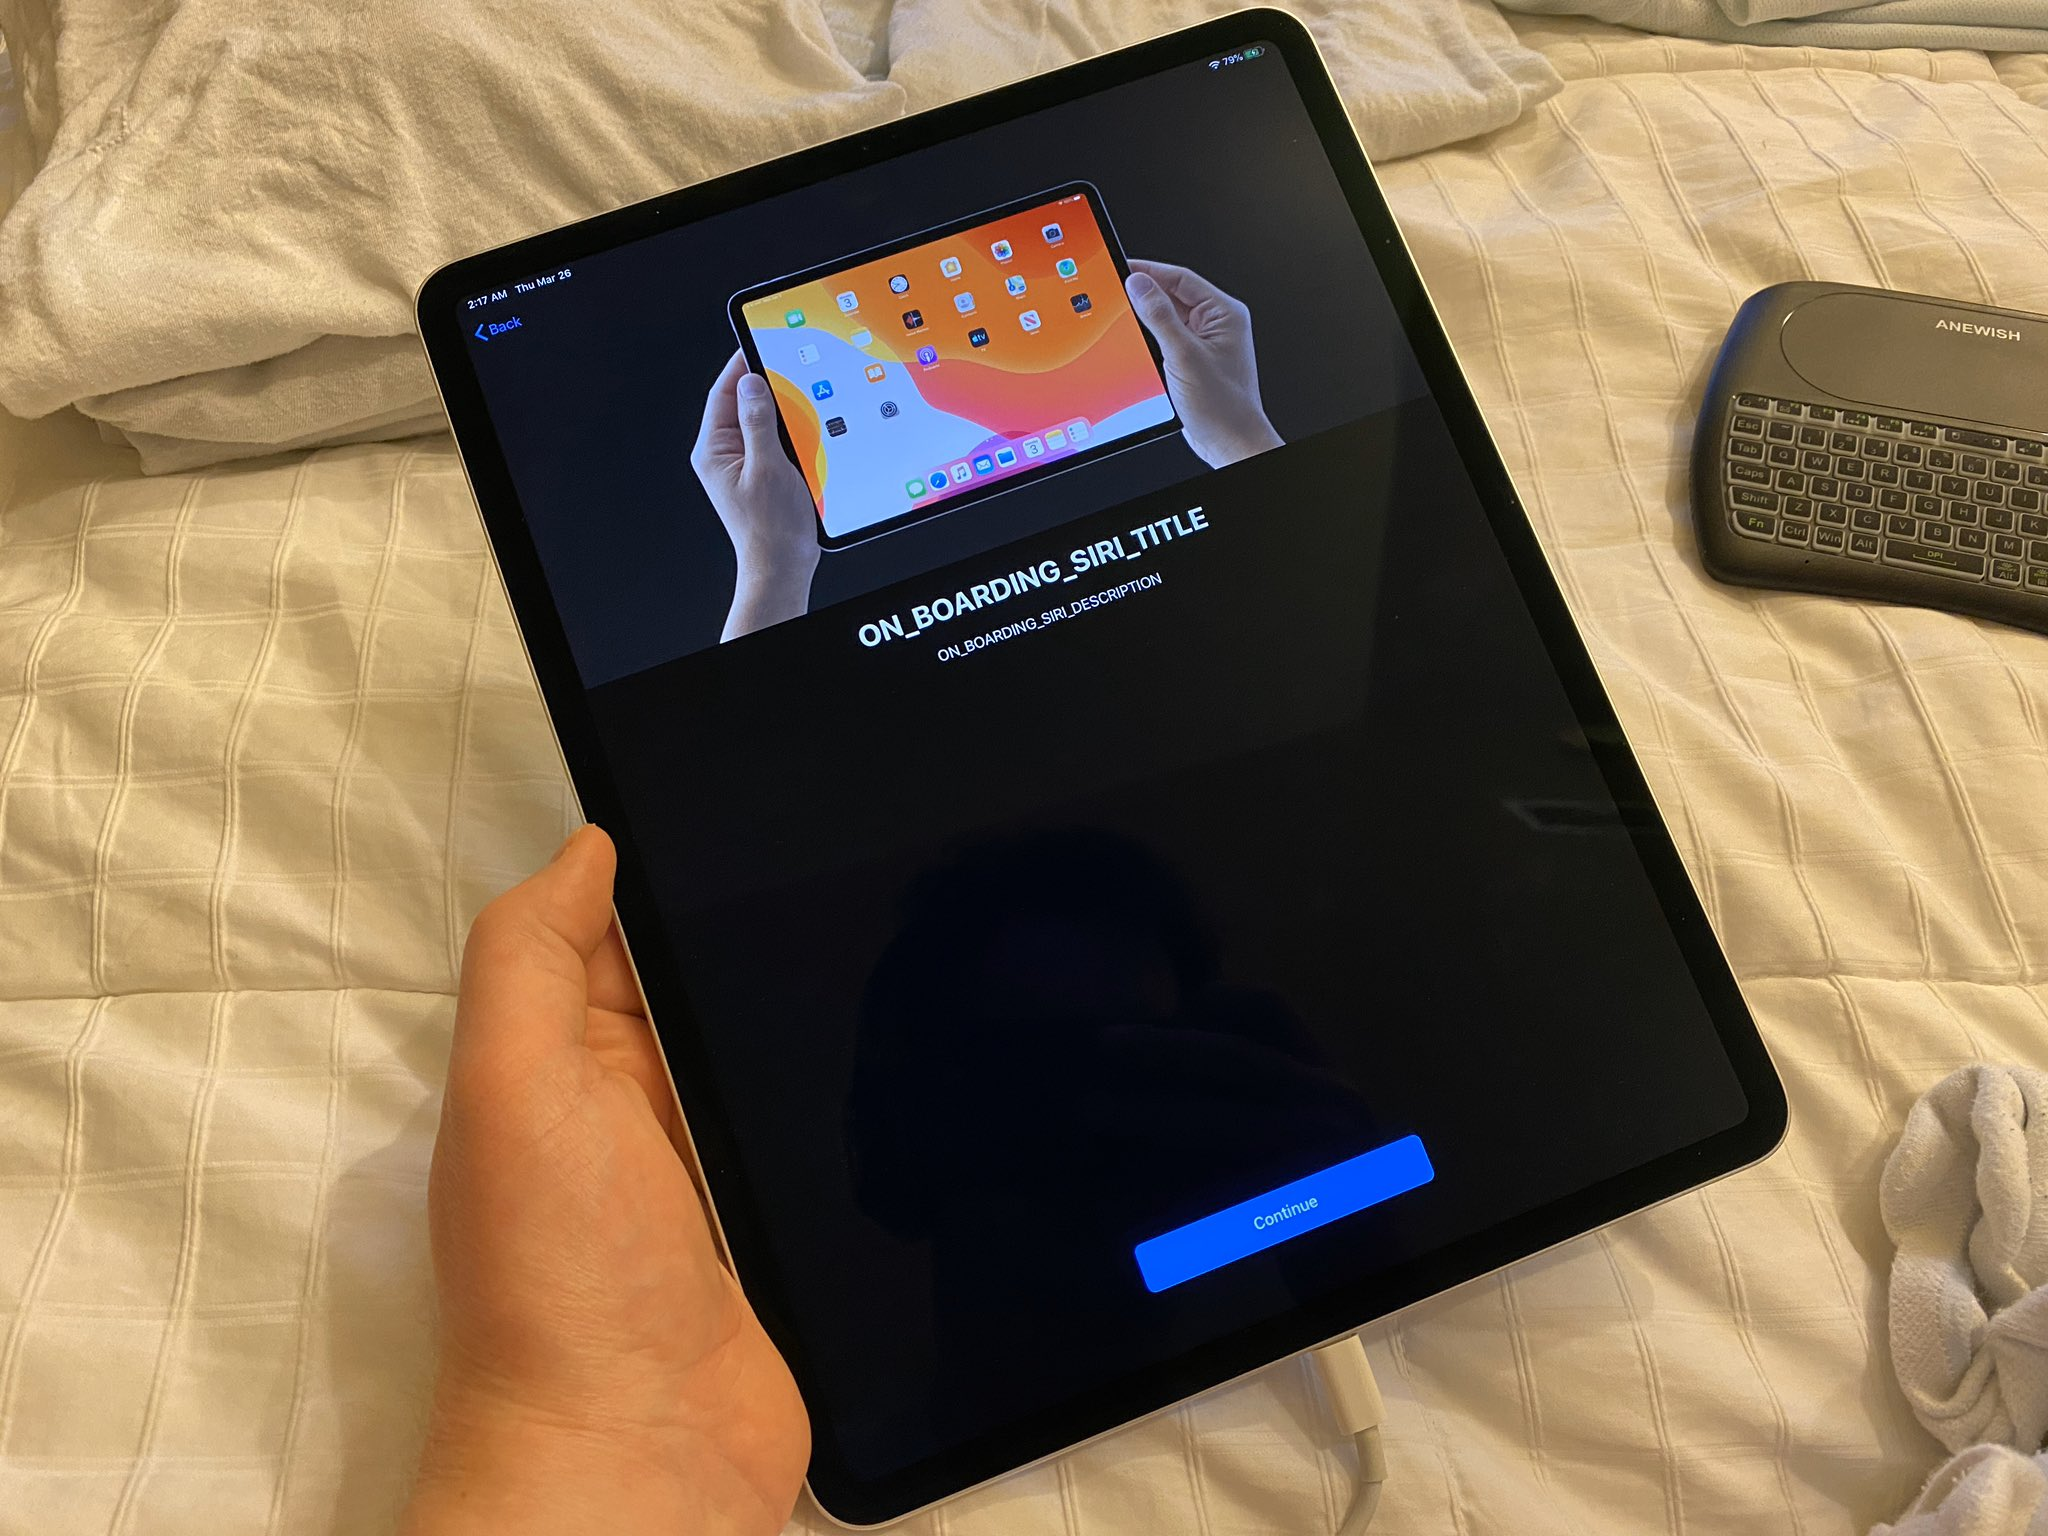
\includegraphics[width=.7\columnwidth]{onboarding-gone-wrong}
    \caption[Implementatiefout bij onboarding]{Bij de ingebruikname van de nieuwe~\href{https://www.apple.com/ipad-pro/}{Apple iPad Pro} werd de onboarding onderbroken door een programmeerfout}
    \label{fig:onboarding:fout}
\end{figure}

\subsection{Welkomstberichten}
\label{sec:onboarding:welkomstberichten}

\textcite{Balboni2018} groepeerde verschillende implementaties van onboarding in acht~\acrshort{acr:ui}/\acrshort{acr:ux} patronen. Wanneer je je net registreerde of wanneer je een nieuwe app open doet op een mobiel toestel heb je zeker al eens een welkomstbericht ontvangen. Negen op tien onboarding-ervaringen starten met een bericht waarin ze de nieuwe klant verwelkomen. Vaak wordt dit bericht ondersteund door een CTA-knop (Call To Action) waarin men bijvoorbeeld de gebruiker kan uitnodigen om deel te nemen aan een rondleiding doorheen de applicatie.

\begin{figure}[h!]
    \centering
    
\includegraphics[width=.3\columnwidth]{onboarding-welkom}
    \caption[Voorbeeld welkomstbericht]{Een welkomstbericht na registratie bij~\href{https://www.headspace.com/}{Headspace}}
    \label{fig:onboarding:welkom}
\end{figure}

\subsection{Rondleidingen}
\label{sec:onboarding:rondleidingen}

Een rondleiding doorheen de applicatie toont alle belangrijke elementen en functionaliteiten even aan met een beknopte uitleg. De rondleiding moet zich echter beperken tot de belangrijkste onderdelen zodat de eindgebruiker zich niet verveeld of geïrriteerd voelt. Bij de rondleiding maakt men veelal gebruik van tooltips (zie figuur~\ref{fig:onboarding:rondleiding}).

\begin{figure}[h!]
    \centering
    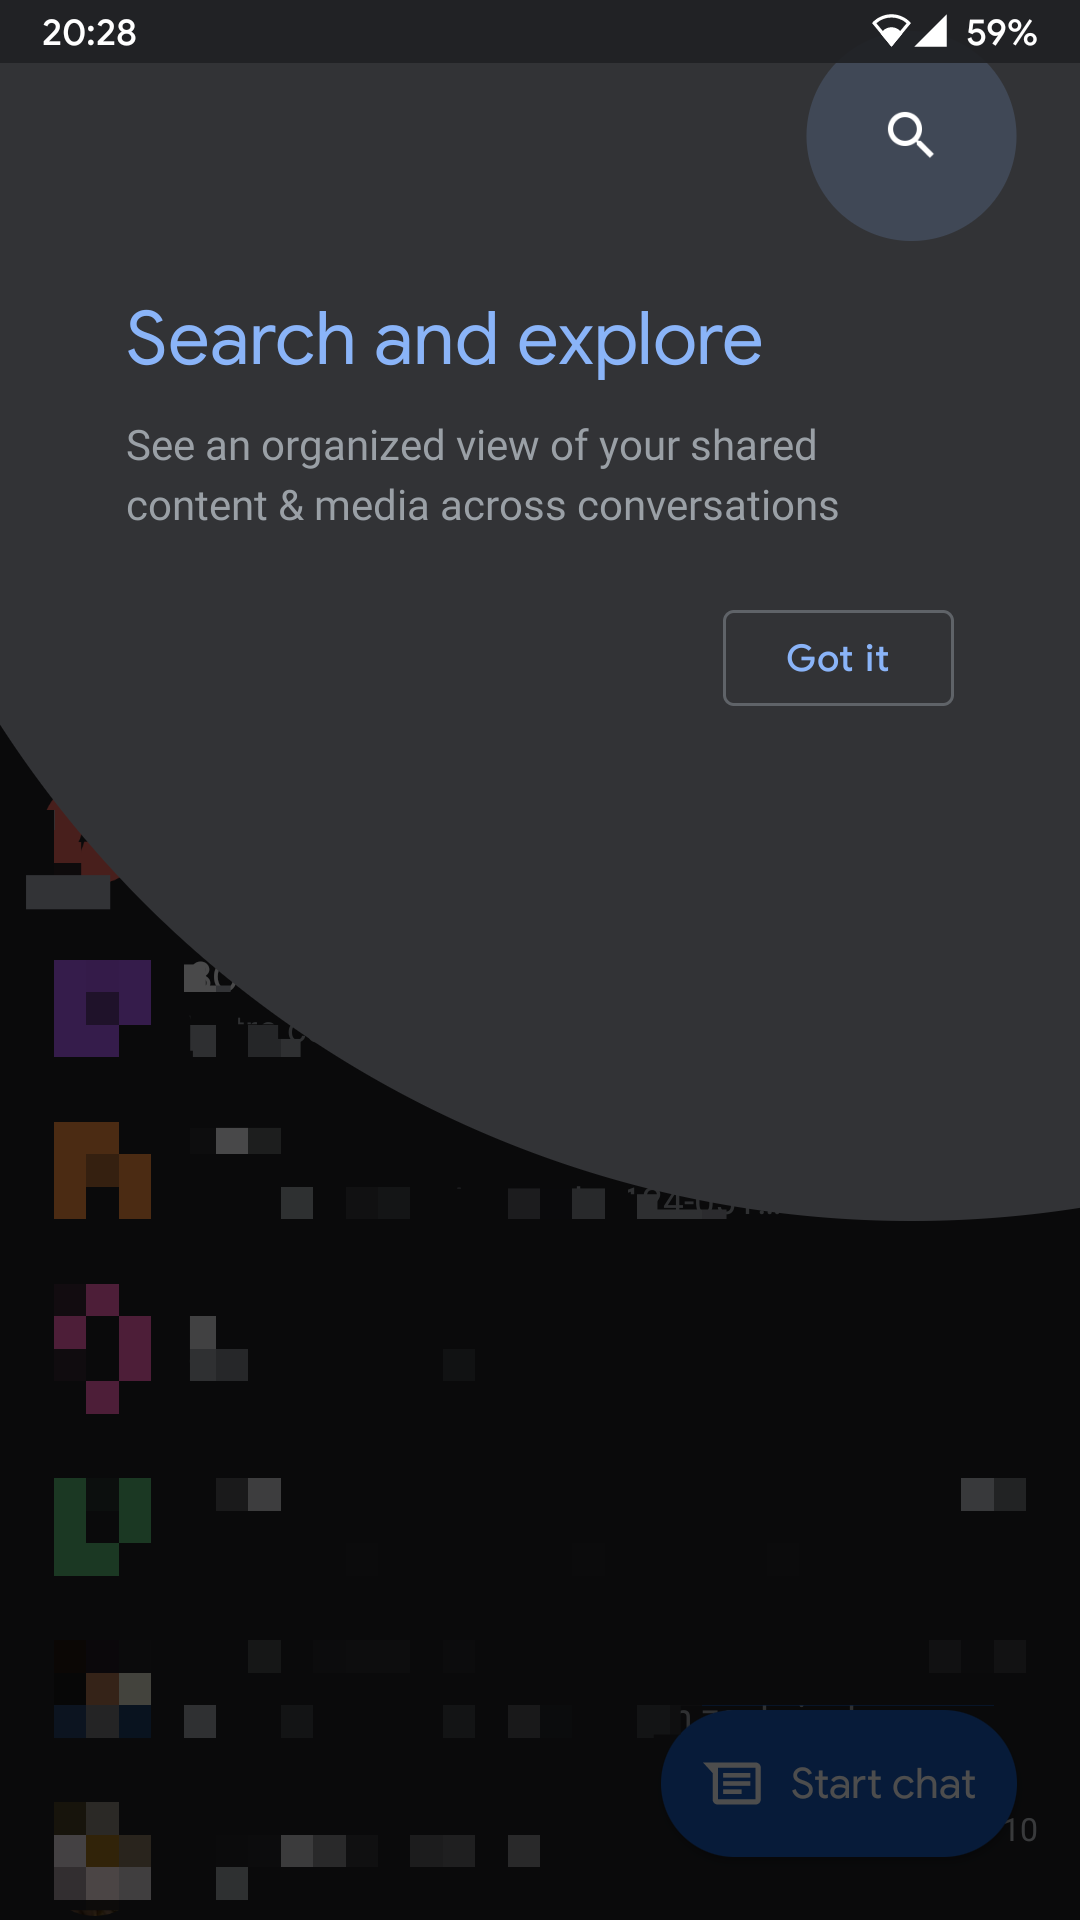
\includegraphics[width=.3\columnwidth]{onboarding-tooltip}
    \caption[Voorbeeld tooltip]{Een tooltip om de zoekfunctie te benadrukken in de~\href{https://messages.google.com/}{Messages} applicatie van Google}
    \label{fig:onboarding:rondleiding}
\end{figure}

Bij grote applicaties of software met een aanzienlijke hoeveelheid aan functies worden de rondleidingen gewoonlijk opgesplitst. Zo leert de gebruiker stap voor stap alle functionaliteit. Wanneer een applicatie een nieuwe functionaliteit toevoegt of een deel van de~\acrshort{acr:ui} wijzigt door middel van een update wordt er vaak een nieuwe rondleiding aangeboden. Zo werd de \href{https://www.theverge.com/2020/3/18/21184865/slack-redesign-update-sidebar-changes-available-now-download}{communicatie-tool Slack in maart 2020 geüpdatet} en werd er voor bestaande gebruikers opnieuw een rondleiding doorheen de wijzigingen gegeven (zie figuur~\ref{fig:onboarding:rondleiding-slack}).

\begin{figure}[h!]
    \centering
    \subfloat[Melding over de update]{{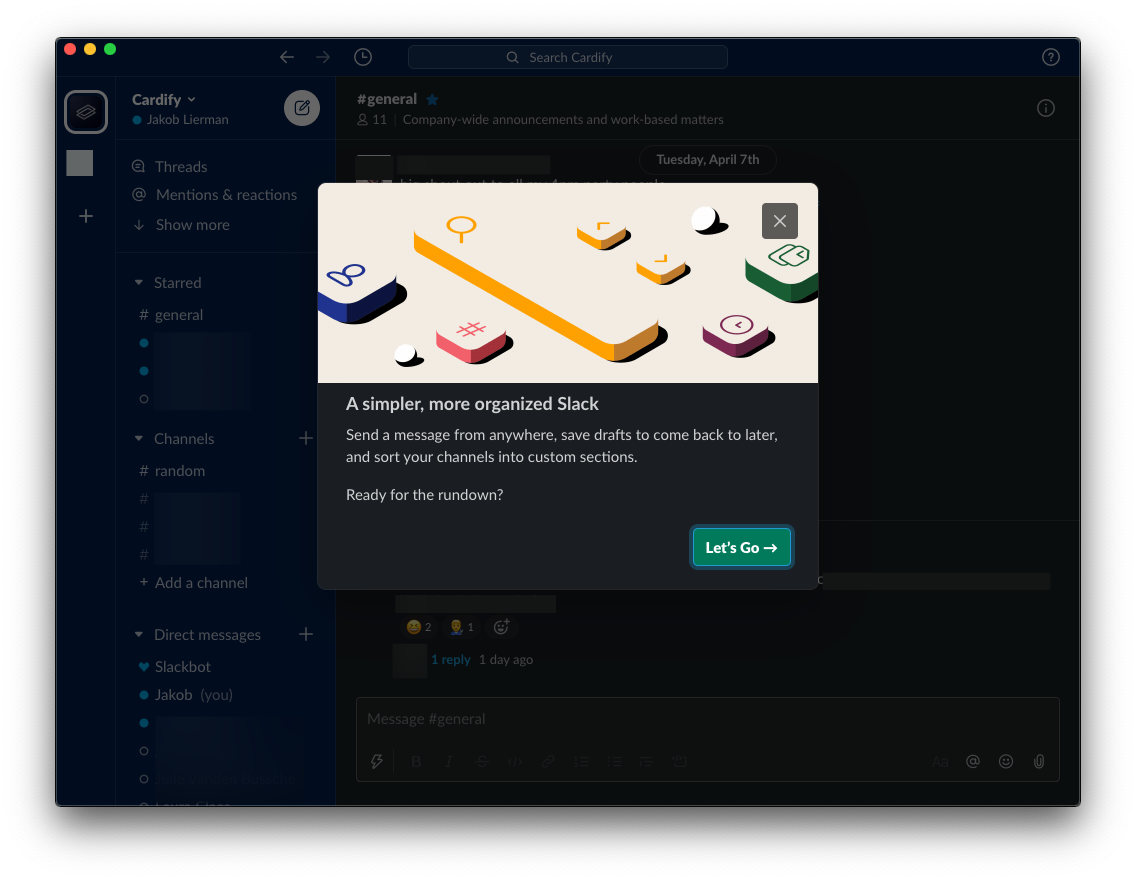
\includegraphics[width=.47\columnwidth]{onboarding-slack-1}}}
    \qquad
    \subfloat[Slack duidt de belangrijkste wijzigingen aan]{{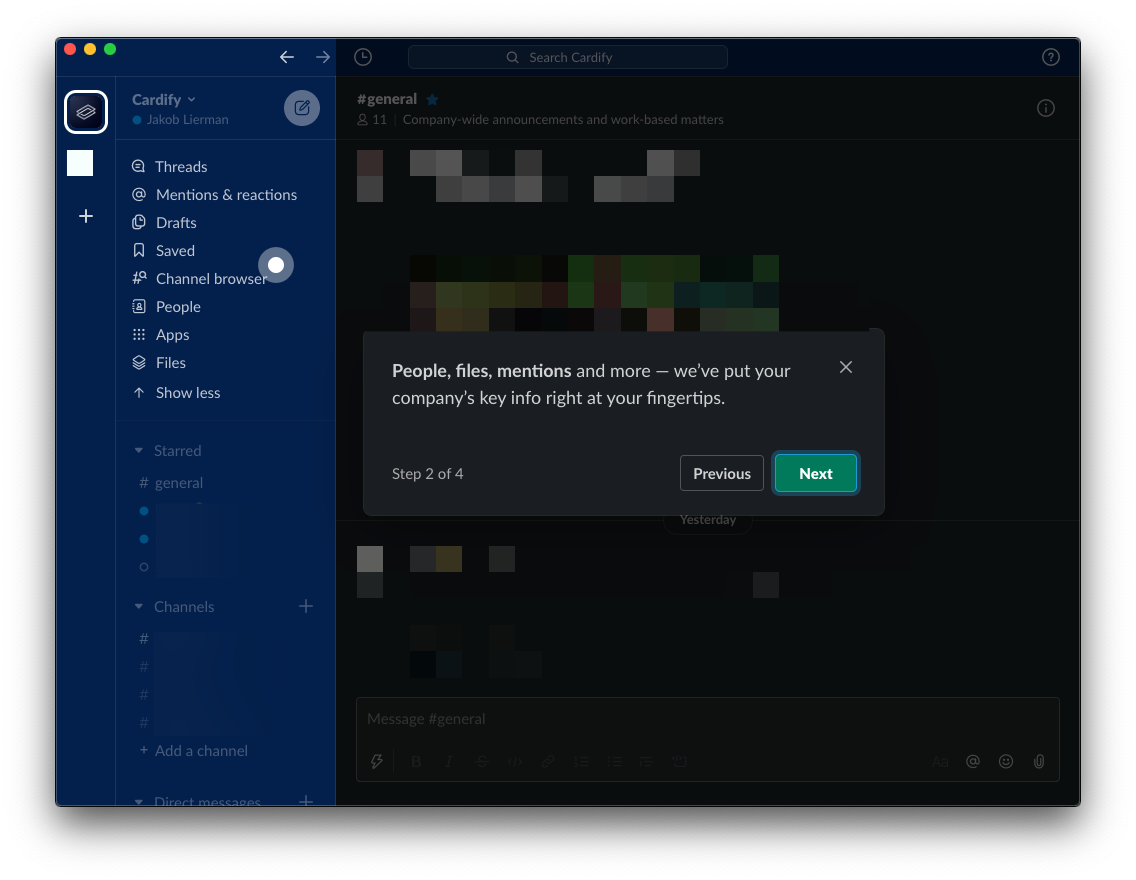
\includegraphics[width=.47\columnwidth]{onboarding-slack-2}}}
    \caption[Voorbeeld rondleiding Slack]{Slack (\url{https://slack.com/}) gaf bestaande gebruikers de kans om nieuwe functies te ontdekken door middel van een rondleiding na een update van de applicatie}
    \label{fig:onboarding:rondleiding-slack}
\end{figure}

\subsection{Voortgangsindicatoren}
\label{sec:onboarding:voortgang}

De mens wil opdrachten voltooien. Zeker wanneer men de voortgang kan opvolgen. Doorheen het volledige onboarding-proces kan de voortgang dus weergegeven worden in voortgangsbalken of voortgangsstippen (zie figuur~\ref{fig:onboarding:voortgang}).

\begin{figure}[h!]
    \centering
    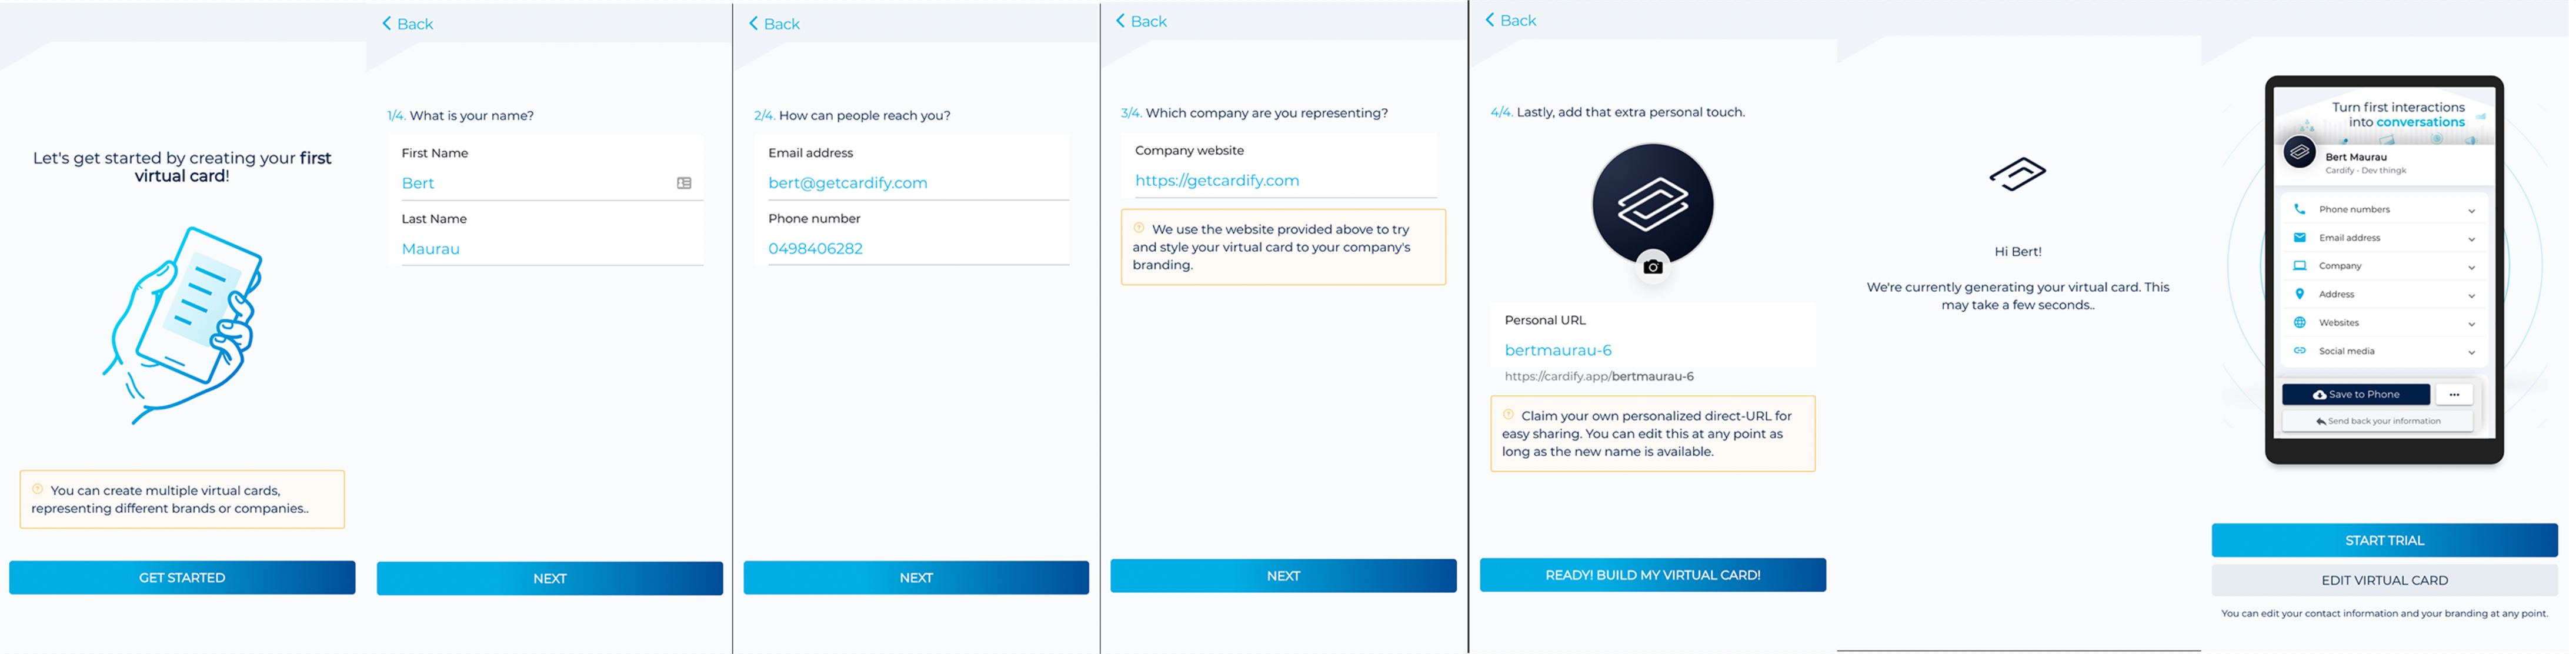
\includegraphics[width=\columnwidth]{cardify-onboarding-app}
    \caption[Voorbeeld voortgangsindicatoren]{Weergave van resterende stappen bij de registratie in de Cardify applicatie}
    \label{fig:onboarding:voortgang}
\end{figure}

\subsection{Checklists}
\label{sec:onboarding:checklists}

Checklists zetten net zoals voortgangsindicatoren aan tot het voltooien van opdrachten. Het afwerken van een item in de checklist geeft de gebruiker een gevoel van voldoening. Checklists worden naar gewoonte ingezet voor complexere taken met meerdere stappen.

\begin{figure}[h!]
    \centering
    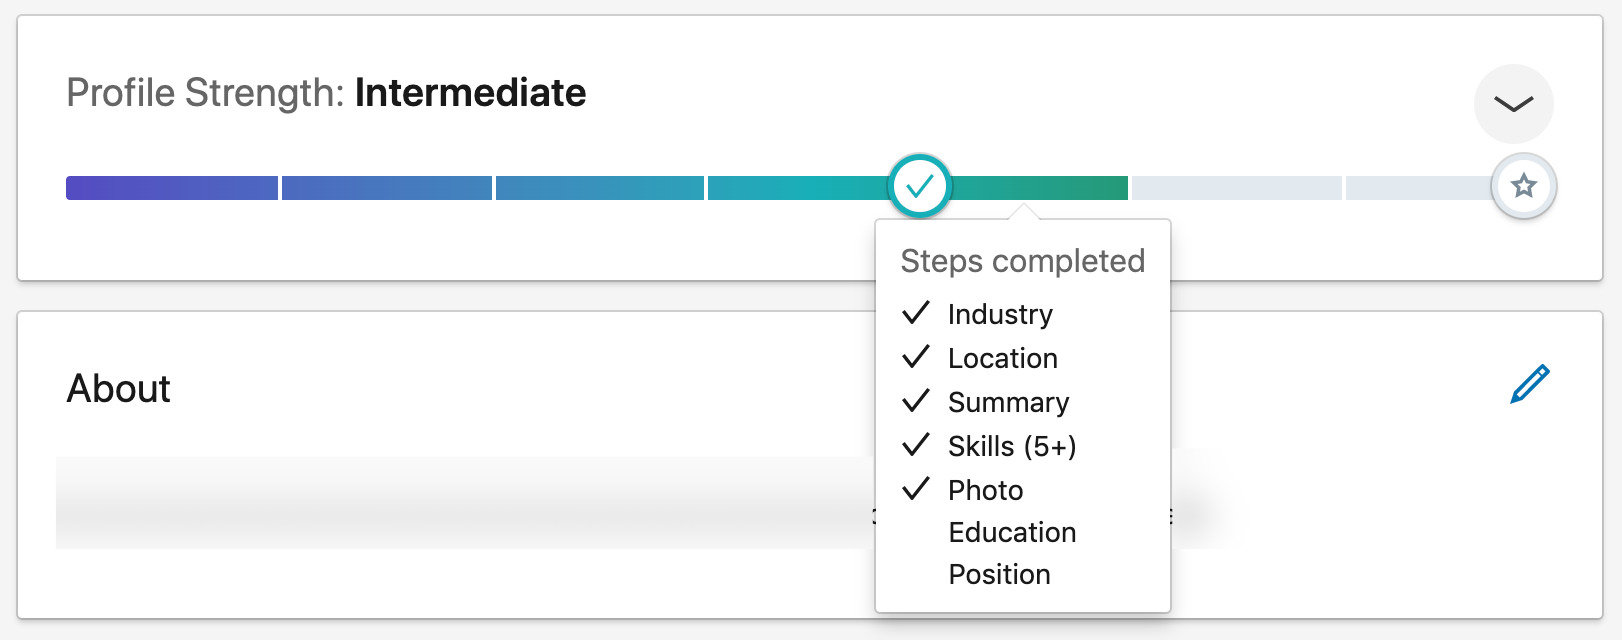
\includegraphics[width=.6\columnwidth]{onboarding-checklist}
    \caption[Voorbeeld checklist]{Checklist bij het vervolledigen van een profiel op~\href{https://www.linkedin.com/}{LinkedIn}}
    \label{fig:onboarding:checklist}
\end{figure}

\subsection{Hotspots}
\label{sec:onboarding:hotspots}

Hotspots zijn gelijkaardig aan de tooltips uit de rondleidingen (zie hoofdstuk~\ref{sec:onboarding:rondleidingen}). De tooltips zijn niet vrijblijvend, een gebruiker die snel aan de slag wil zal hier dus snel door klikken zonder veel informatie opgenomen te hebben. Hotspots spelen hierop in door zones te creëren waarin de gebruiker kan klikken om meer informatie te verkrijgen over dat~\acrshort{acr:ui}-element of die functionaliteit. Doordat deze hotspots vrijblijvend zijn verhinderen ze de workflow van de gebruiker niet.

\begin{figure}[h!]
    \centering
    \subfloat[Hotspot toont aan waar actie mogelijk is]{{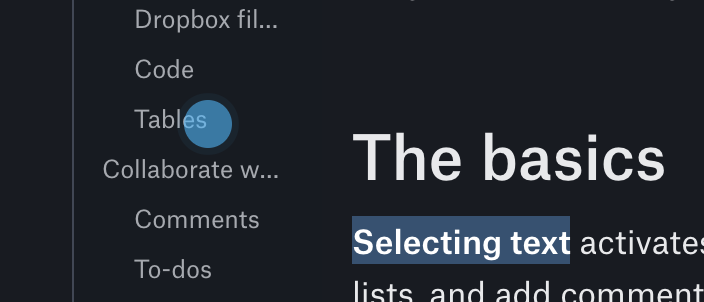
\includegraphics[width=.4\columnwidth]{onboarding-hotspot-1}}}
    \qquad
    \subfloat[Actieve hotspot]{{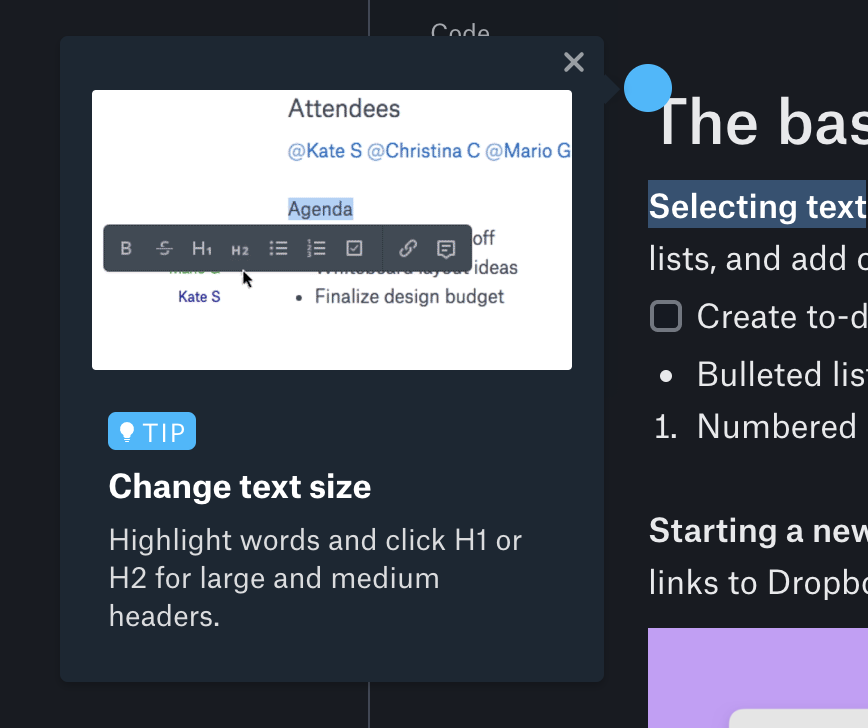
\includegraphics[width=.4\columnwidth]{onboarding-hotspot-2}}}
    \caption[Voorbeeld hotspots]{Hotspots bij ingebruikname van~\href{https://www.dropbox.com/paper}{Dropbox Paper}}
    \label{fig:onboarding:hotspots}
\end{figure}

\subsection{Actie-gedreven tooltips}
\label{sec:onboarding:actie-tooltips}

Actie-gedreven tooltips hebben veel weg van de tooltips uit hoofdstuk~\ref{fig:onboarding:rondleiding}. Het verschil zit hem in de interactie ermee. Een eenvoudige tooltip bevat een omschrijving of uitleg en een knop om de tooltip te sluiten of om naar de volgende te gaan in de rondleiding. Bij actie-gedreven tooltips moet men een kleine opdracht uitvoeren, zoals op een knop klikken of tekst invoeren. De bedoeling hiervan is dat men bijleert hoe de applicatie in zijn werk gaat door deze ook echt te gebruiken. In onderzoek van~\textcite{Oliveira2019} toont hij zelfs aan dat deze tooltips een beter effect hebben dan de eenvoudige tooltips van een rondleiding.

Dit kan ook ingezet worden in een bedrijfsomgeving. Een nieuwe werknemer die nog moet leren werken met de vele functionaliteiten van (de software van) een machine zal met deze hands-om mentaliteit veel vlotter zelfstandig aan de slag kunnen gaan.

\subsection{Uitgestelde accountcreatie}
\label{sec:onboarding:uitgestelde-accountcreatie}

Uitgestelde accountcreatie stelt, zoals je uit de benaming al kon afleiden, de accountcreatie uit. Hierbij worden eerst de functionaliteiten van de software aangehaald voordat de gebruiker zicht hoeft te registreren. Dit beperkt het aantal velden dat de gebruiker moet invullen bij het eerste contact met de applicatie. De gebruiker moet nadien wel in de juiste richting geduwd worden zodat deze toch de registratie voltooid.

\begin{figure}[h!]
    \centering
    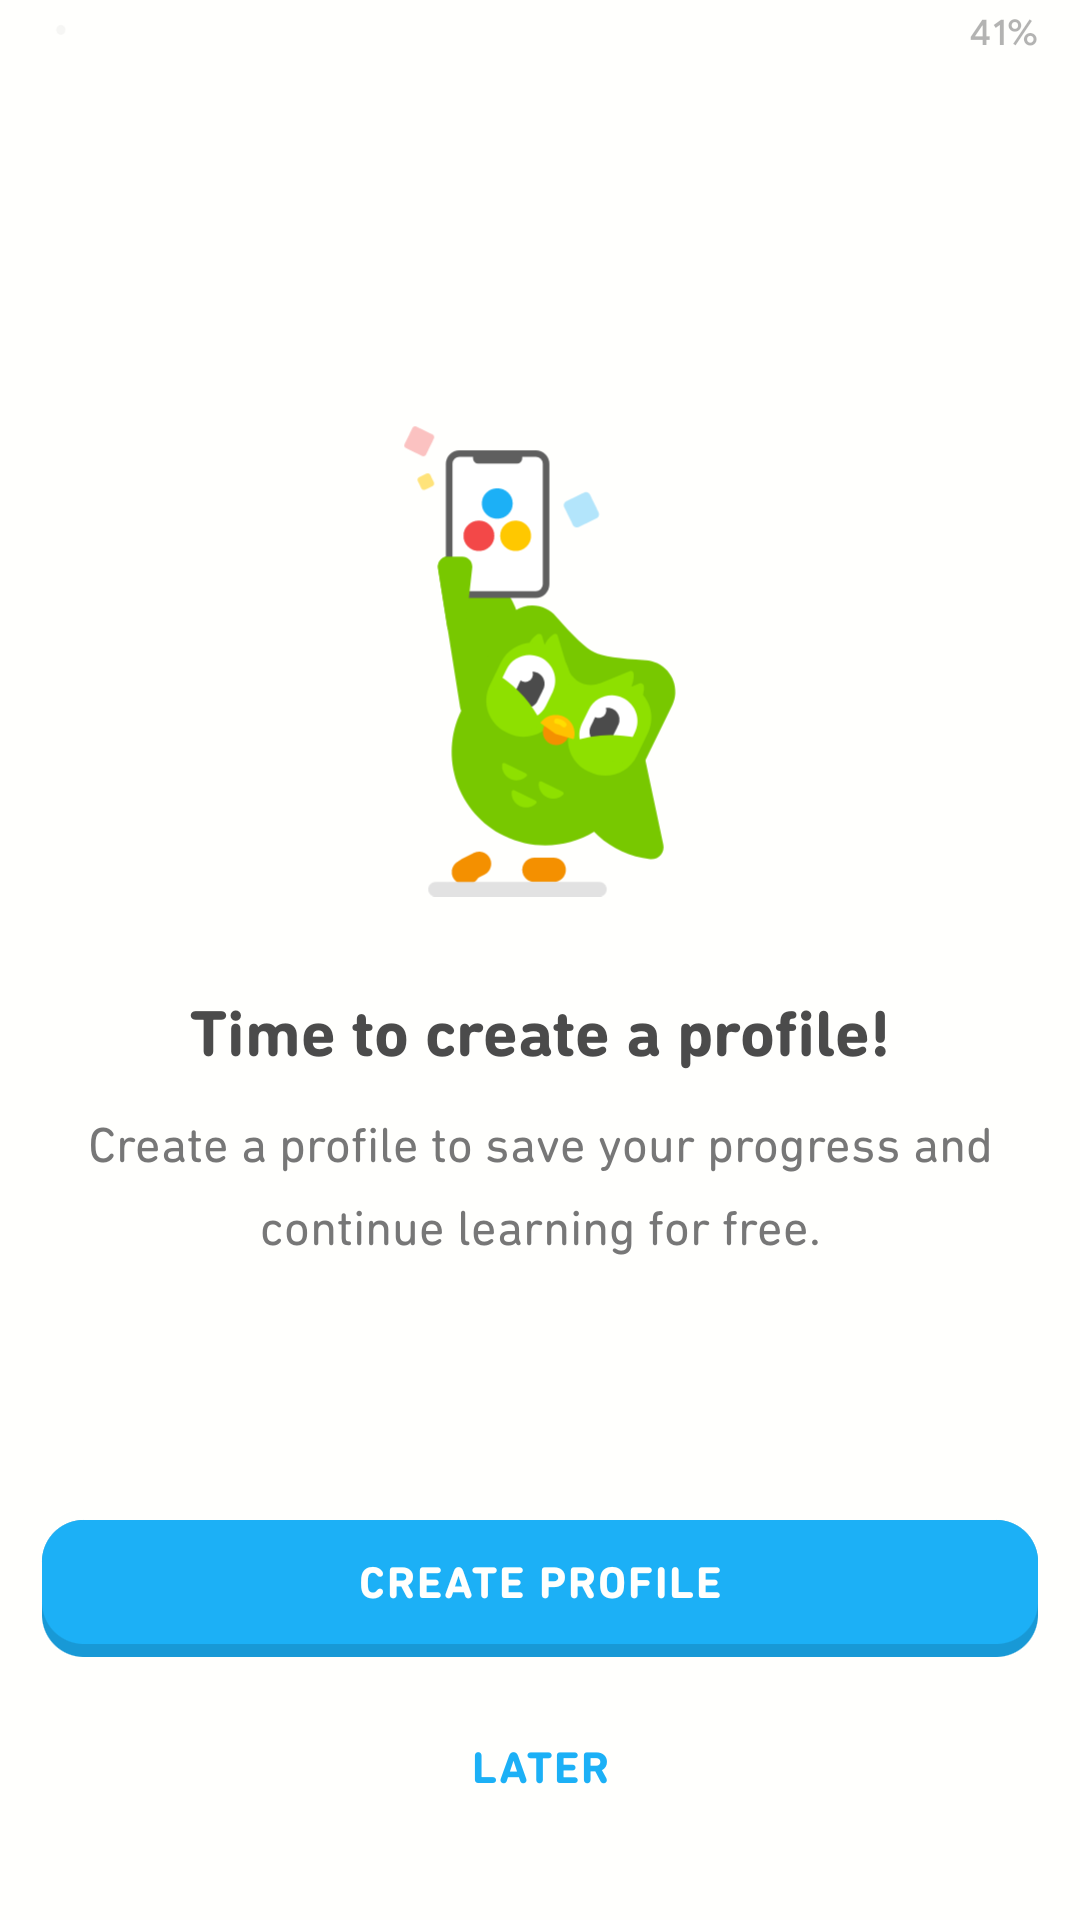
\includegraphics[width=.3\columnwidth]{onboarding-uitstel}
    \caption[Voorbeeld uitgestelde accountcreatie]{\href{https://www.duolingo.com/}{Duolingo} vereist geen account voor de werking van de applicatie, er worden op bepaalde momenten wel meldingen gegeven van de voordelen van een account}
    \label{fig:onboarding:uitgestelde-accountcreatie}
\end{figure}

\subsection{Gepersonaliseerde onboarding}
\label{sec:onboarding:gepersonaliseerd}

Gepersonaliseerde onboarding zorgt ervoor dat de gebruiker bij de eerste ingebruikname van de applicatie meteen een gepersonaliseerde software voor handen heeft. Dit kan door bijvoorbeeld in een kennismakingsformulier de interesses van de gebruiker op te vragen zodat men enkel relevante inhoud krijgt.

\begin{figure}[h!]
    \centering
    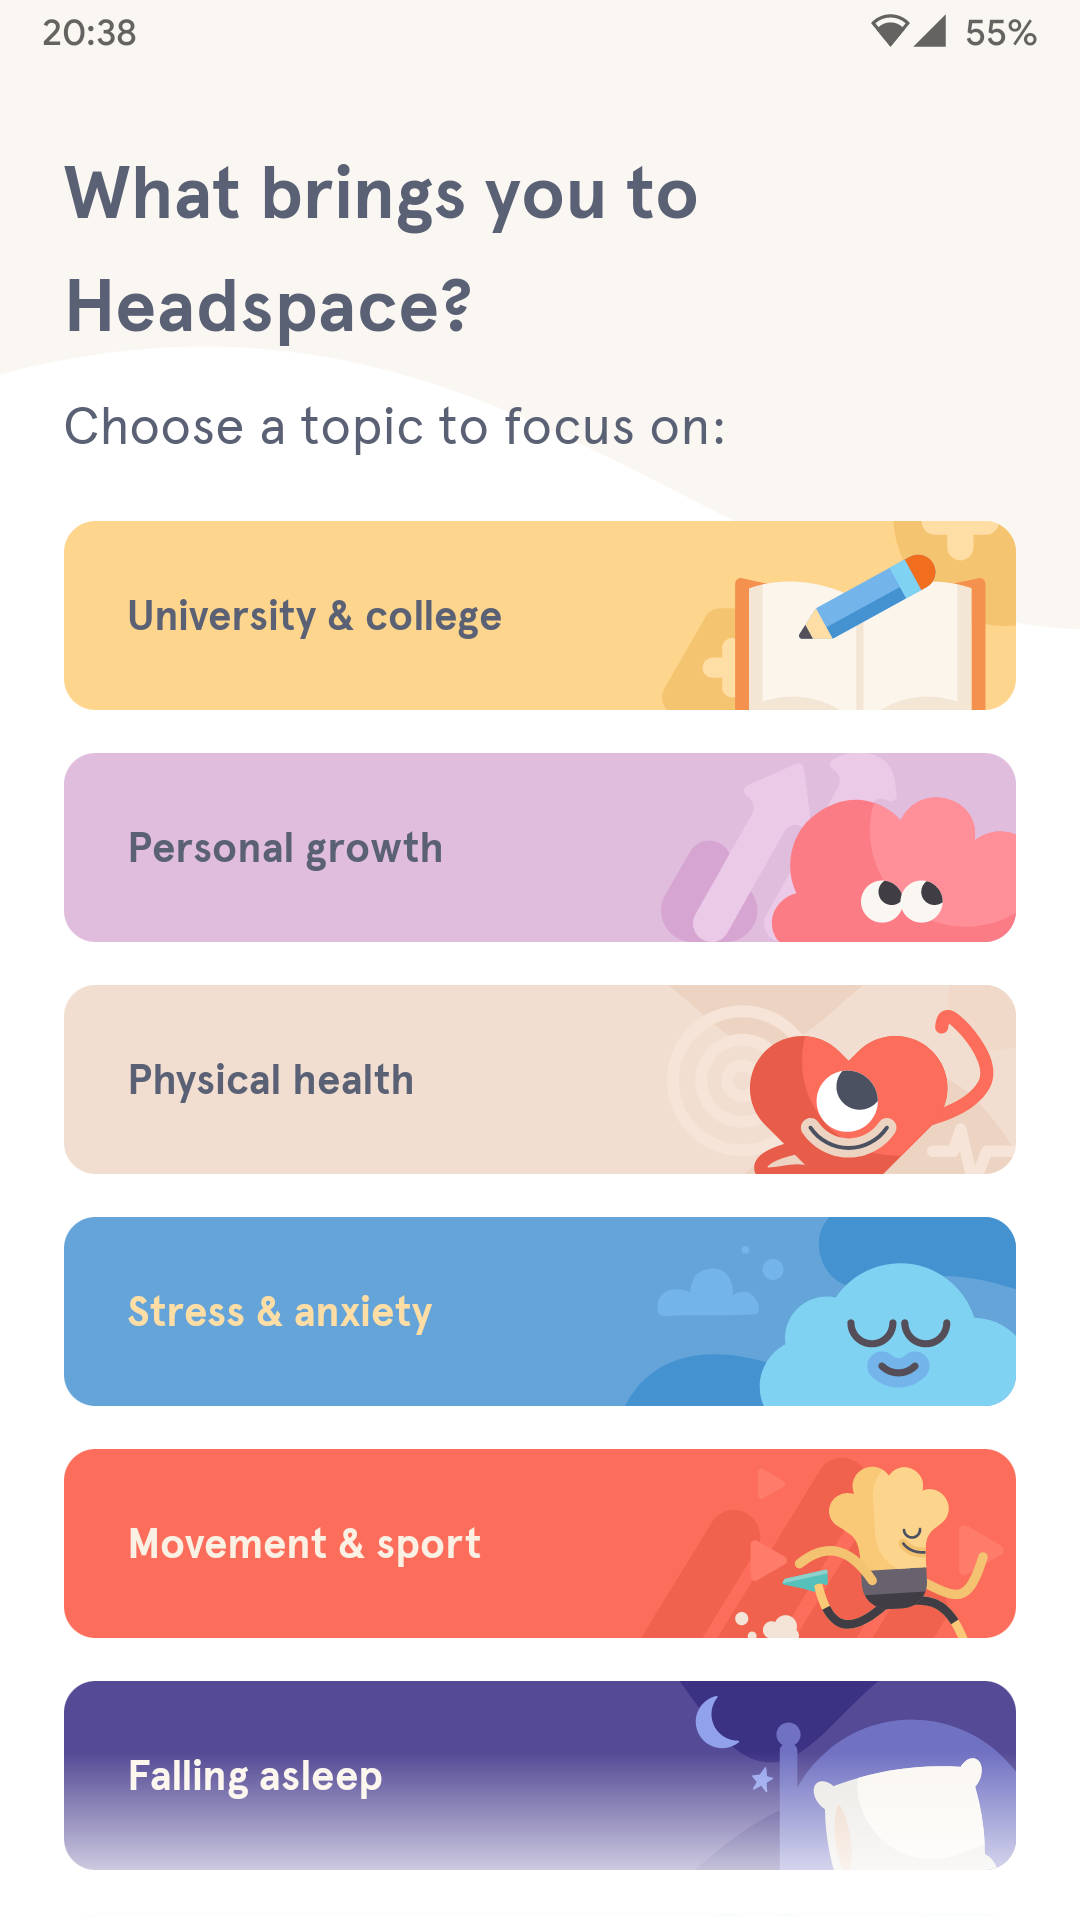
\includegraphics[width=.3\columnwidth]{onboarding-personal}
    \caption[Voorbeeld gepersonaliseerde onboarding]{Een vragenlijst om de verdere ervaring bij \href{https://www.headspace.com/}{Headspace} te personaliseren}
    \label{fig:onboarding:gepersonaliseerd}
\end{figure}

\subsection{Testen van onboarding}
\label{sec:onboarding:testen}

Zoals~\textcite{Strahm2018} verduidelijkten, is de creatie van een onboardingsflow verschillend voor elke applicatie. Het ontwerpen zelf is een iteratief proces waarbij men afwisselt tussen implementatie en testen. Hier komt laboratory testing zeker van pas (zie hoofdstuk~\ref{sec:usability-testing:lab-field-testing}).

De onboarding wordt net zoals andere~\acrshort{acr:ux} en~\acrshort{acr:ui}-elementen getest door middel van usability testing (zie hoofdstuk~\ref{sec:usability-testing}). Hierbij kan rekening gehouden worden met de snelheid waarop een gebruiker een taak kan uitvoeren met behulp van uitleg uit onboarding-technieken. Ook moet gekeken worden naar het gevoel dat de gebruiker heeft bij deze onboarding. Indien bijvoorbeeld het grootste deel van de testpersonen te snel door de rondleiding klikt is deze hoogstwaarschijnlijk te lang. Door te werken met het ``think aloud'' protocol en achteraf gerichte vragen te stellen aan de testpersoon kan men snel inzichten creëren over hoe men deze onboarding-technieken kan verbeteren.

\section{In-app training}
\label{sec:in-app-training}

Eenmaal de onboarding voorbij is kan de gebruiker uiteraard terug vallen op de in-app training. Dit zorgt ervoor dat de gebruiker na de onboarding niet in de steek wordt gelaten. In-app user training kan meerdere vormen aannemen. De meest gekende is een help-sectie in de applicatie of online. Hier kan men antwoorden vinden op veelgestelde vragen. Vaak is er ook een formulier aanwezig om complexere vragen op te sturen.

\begin{figure}
    \centering
    \subfloat[Help in de navigatie]{{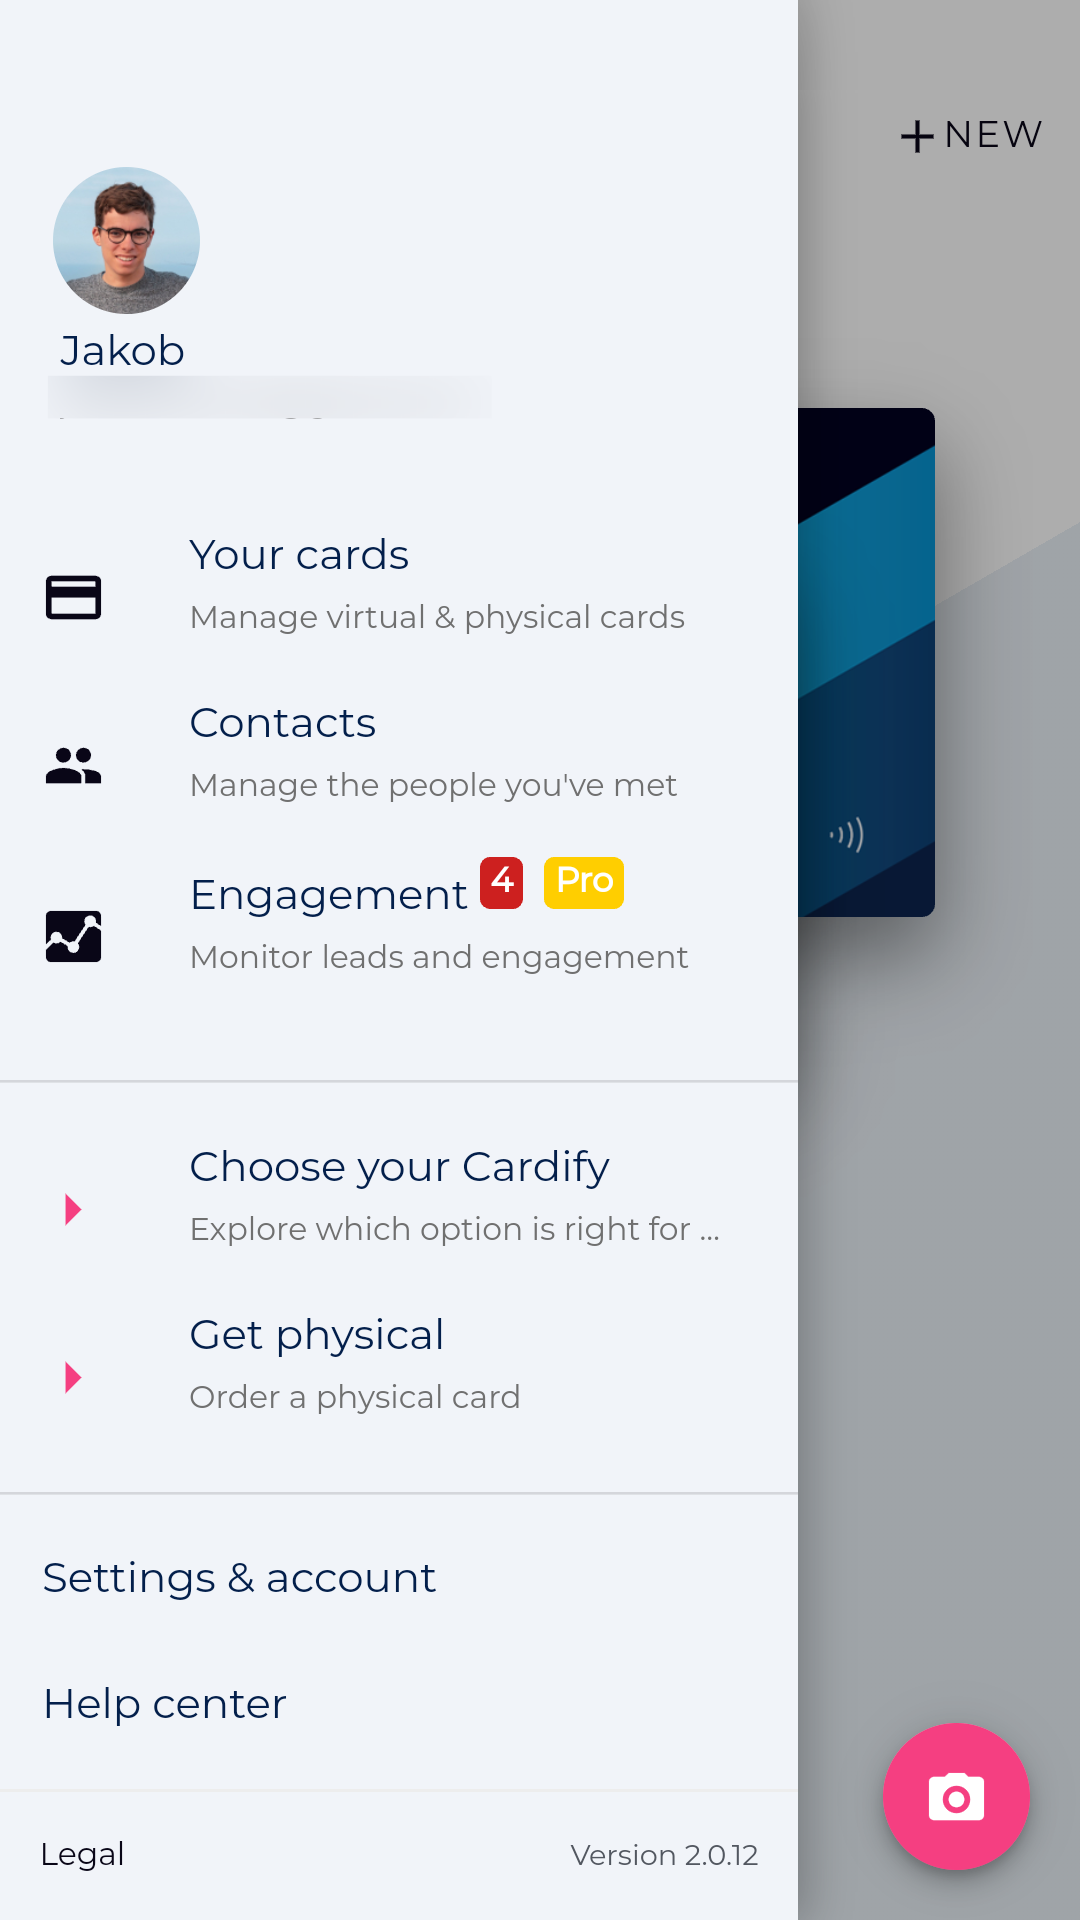
\includegraphics[width=.3\columnwidth]{cardify-help-1}}}
    \qquad
    \subfloat[Help submenu]{{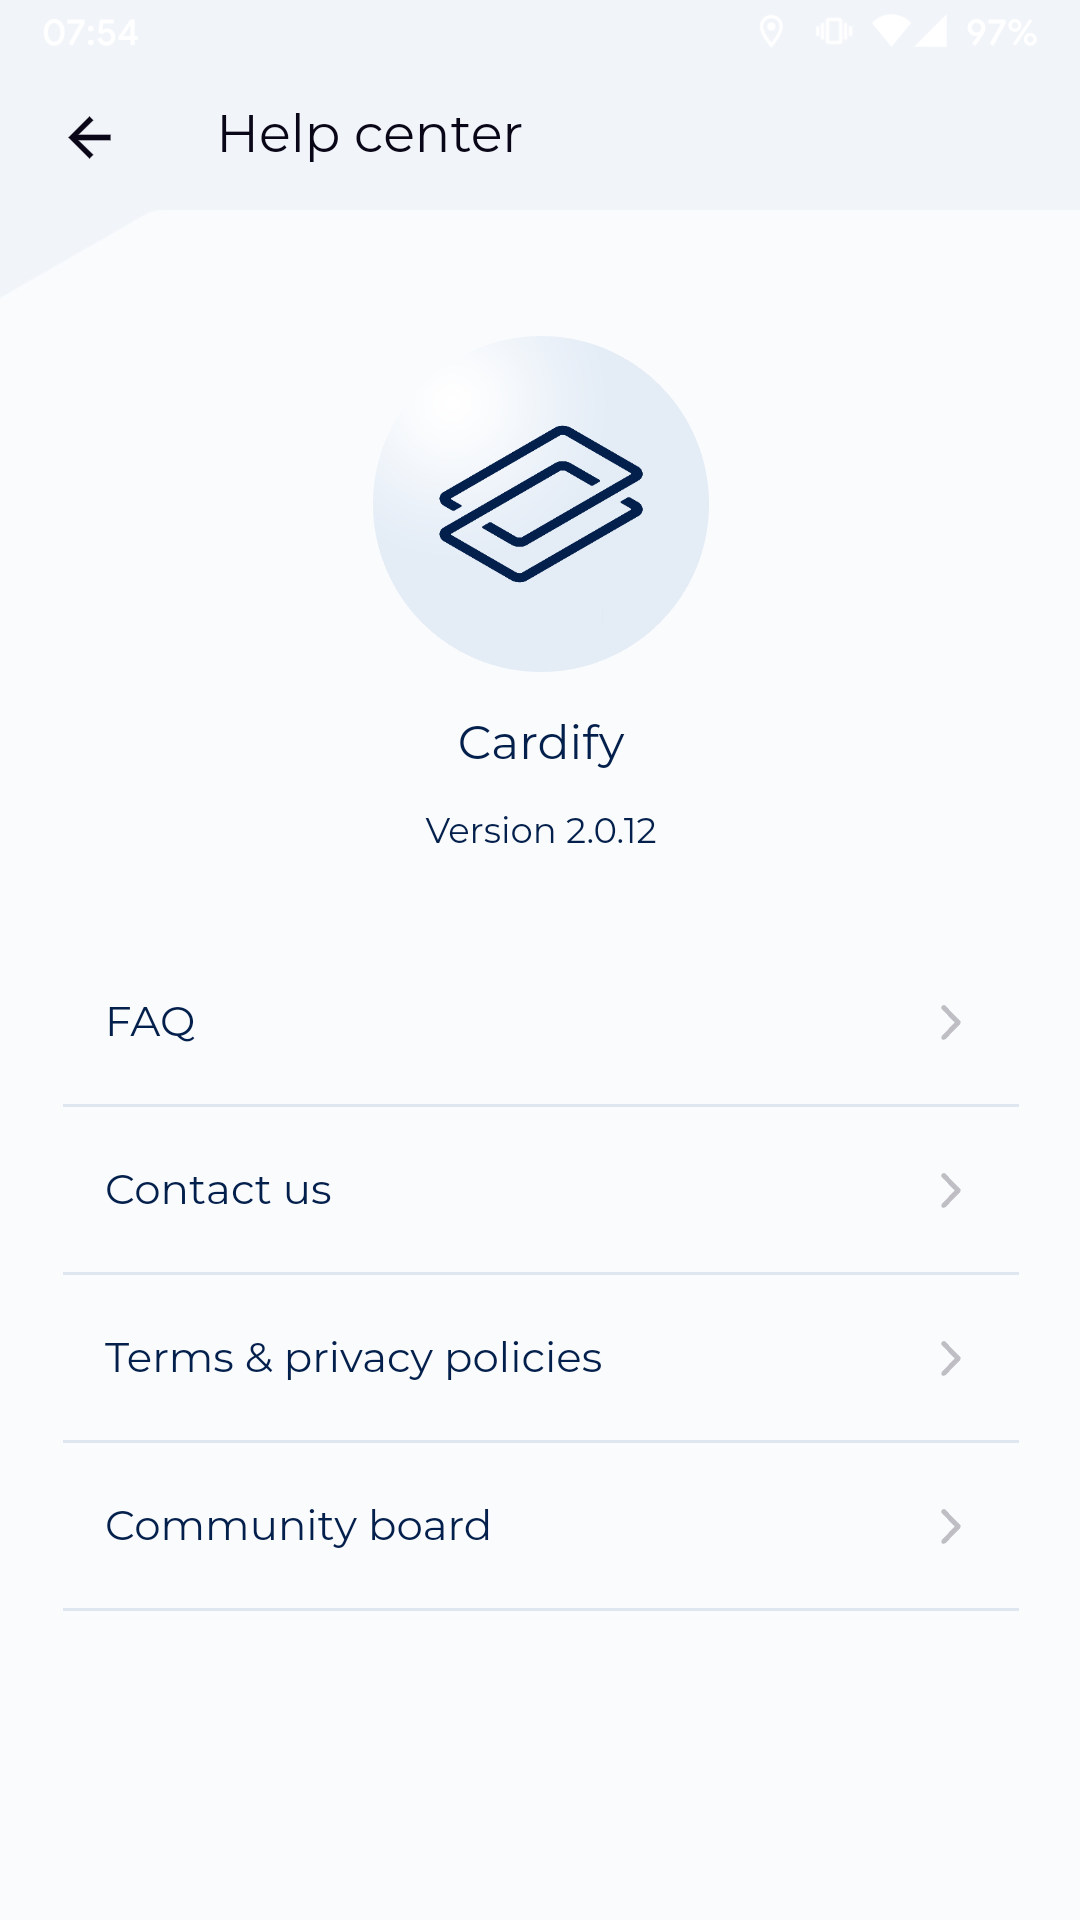
\includegraphics[width=.3\columnwidth]{cardify-help-2}}}
    \caption[Voorbeeld help-sectie]{Help bij Cardify, te vinden op \url{https://help.getcardify.com/}}
    \label{fig:inapptraining:help}
\end{figure}

Tooltips (zie hoofdstuk~\ref{sec:onboarding:rondleidingen}) komen doorheen de applicatie terug. Omdat teveel tooltips bij de ingebruikname van de applicatie geen goed idee zijn, verspreid men deze over de verschillende functionaliteiten van de applicatie. Zo leert de gebruiker gaandeweg meer over de verschillende mogelijkheden.

\section{De verschillen tussen~\acrshort{acr:ux} en~\acrshort{acr:ui}}
\label{sec:ux-vs-ui}

\Glspl{acr:ui} omvatten de ``looks'' van de applicatie. Een~\acrshort{acr:ui} designer vult zijn of haar dag dus met het ontwerpen en schetsen van de interface en verscheidene elementen daarvan~\autocite{Lamprecht2019}.

\epigraph{\acrshort{acr:ux} is focused on the user’s journey to solve a problem,~\acrshort{acr:ui} is focused on how a product’s surfaces look and function.}{\textit{Ken Norton - Partner at Google Ventures, Ex-Product Manager at Google}}

Terwijl het bij~\acrshort{acr:ux} design steeds om het vinden en oplossen van gebruiksproblemen gaat heeft~\acrshort{acr:ui} design daar weinig mee te maken. Bij~\acrshort{acr:ui} design ligt de focus op het creëren van esthetisch mooie interfaces. Het ontwerpen van~\glspl{acr:ui} wordt meestal vooraf gegaan door het~\acrshort{acr:ux} ontwerpproces. Terwijl~\acrshort{acr:ux} van toepassing is op alle soorten producten en diensten, is~\acrshort{acr:ui} enkel van toepassing op digitale producten.

\acrfull{acr:ux} en~\acrfull{acr:ui} gaan hand in hand. Zonder een goed uitgewerkt~\acrshort{acr:ux} design mag de~\acrshort{acr:ui} nog zo goed zijn, de gebruikers zullen steeds problemen ondervinden bij het gebruik van de applicatie. Het omgekeerd geldt natuurlijk ook.

\subsection{Software voor~\acrshort{acr:ui} design}
\label{sec:ux-vs-ui:software}

Ontwerpen van interfaces kan vele vormen aannemen. Van een schets op papier tot een prototype waarin men zelfs enkele navigatie elementen kan nabootsen. Softwarepakketten populair bij~\acrshort{acr:ui} designers bevatten momenteel \href{https://www.adobe.com/products/photoshop.html}{Adobe Photoshop}, \href{https://www.sketch.com/}{Sketch} en \href{https://www.figma.com/}{Figma}.

\begin{figure}[h!]
    \centering
    \subfloat[Schets op papier]{{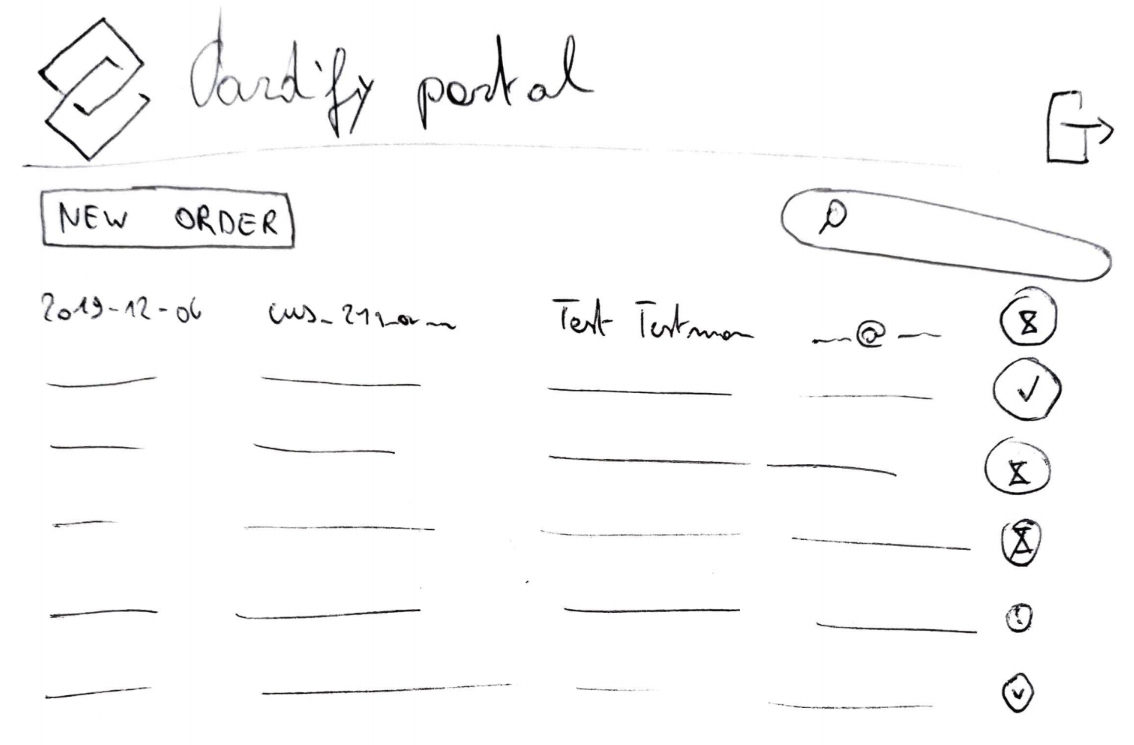
\includegraphics[width=.36\columnwidth]{ui-papier}}}
    \qquad
    \subfloat[Figma]{{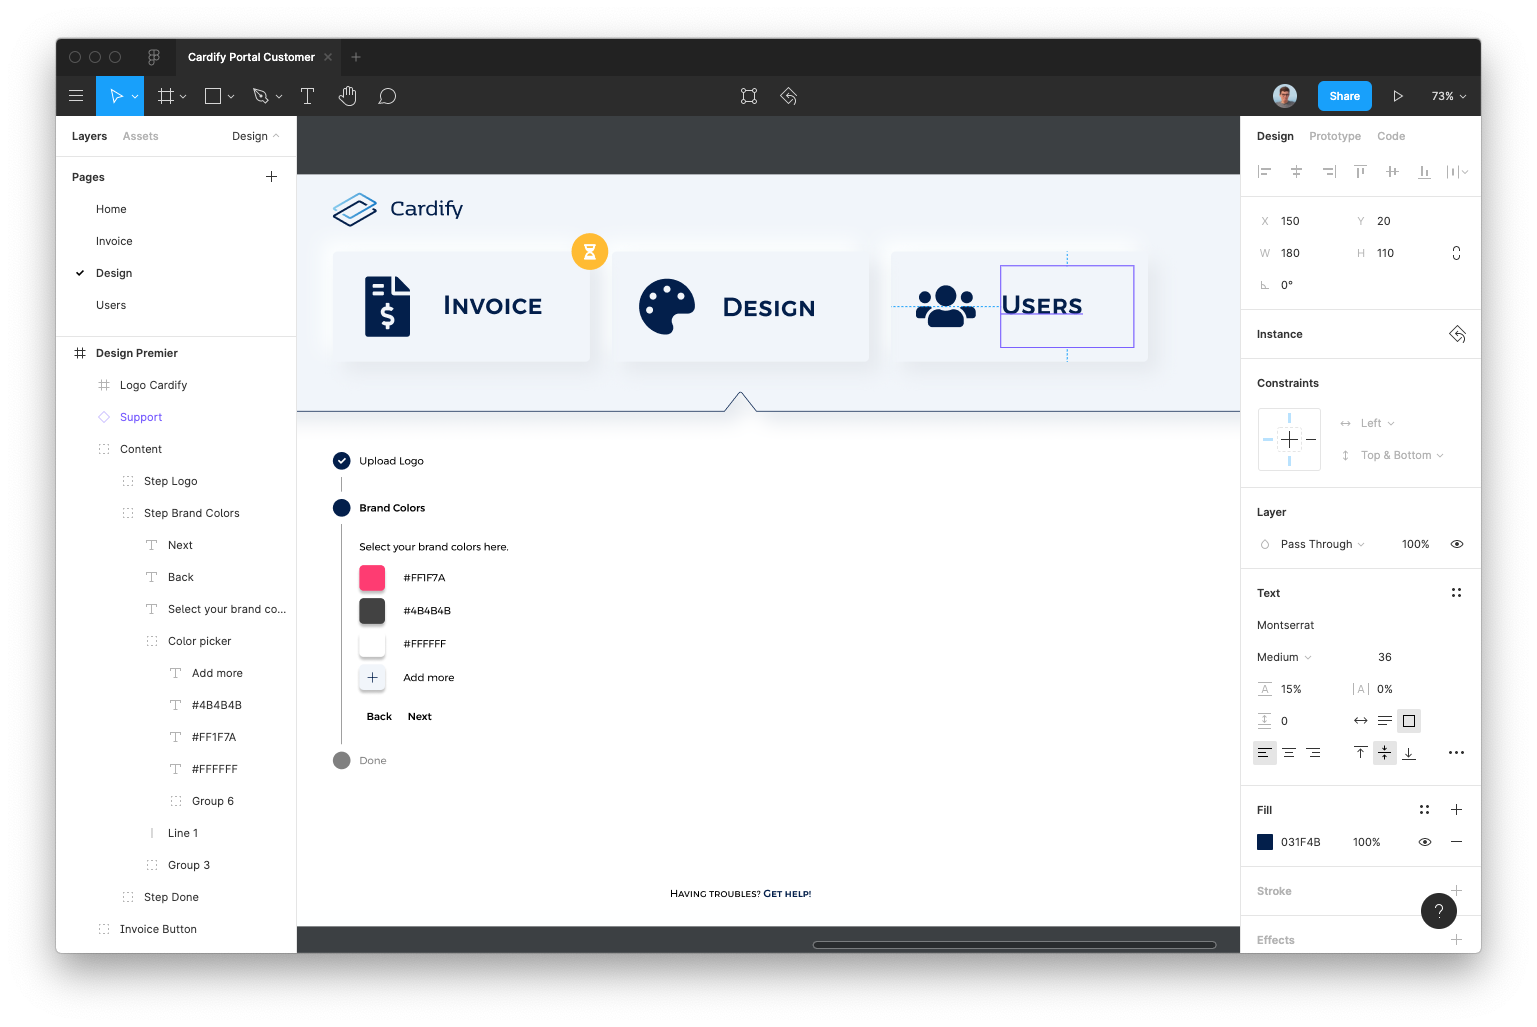
\includegraphics[width=.5\columnwidth]{ui-software}}}
    \caption[Voorbeeld \acrshort{acr:ui}-designproces]{\acrshort{acr:ui} design van \href{https://office.getcardify.com/}{Cardify Office}}
    \label{fig:ux-vs-ui:software}
\end{figure}
